\chapter{Accuracy in Optical Tracking with Fiducial Markers using Condition Number}
\label{chap:Accuracy in Optical Tracking with Fiducial Markers using Condition Number}

%New chapter
In this thesis we only consider the planar control points.
It was already proven that a square is a very stable and robust configuration for all camera poses in planar fiducial markers. Using four optimal control points with maximal equal distance to each other has the biggest influence on the improvement of accuracy\cite{dynamic_markers}.
Based on this conclusion, we also placed four control points on a planar visual fiducial marker, which are set as features in the world coordinate system.

We already know that the optical tracking with fiducial markers is commonly used in robotic applications or in augmented reality systems. One part of our work based on the \textbf{MOMA} odometry system which was shown in figure \ref{fig:moma} was to find the \textbf{accuracy function}. The \textbf{accuracy function} in our case was used to describe the specific distribution of tracking
accuracy dependent on positional relationship(such as distance or angle) between camera and marker. With this \textbf{accuracy function} we can calculate how the robot with camera and marker should be located and oriented, so we can get a optimal camera pose with minimal transformation error($\Delta R, \Delta t$).

%TODO
In previous analysis from other researchers it is already clear proven that the error in homography estimation is dependent on the singular values of the A matrix in the DLT algorithm\cite{chen2009error}.
Furthermore in \cite{dynamic_markers}
there is a research for optimal control point configurations for homography and pose estimation. The authors investigated a approach to find the optimal control point based on condition number of the A matrix in the DLT algorithm. There is a detailed derivation why we can use condition number of the A matrix in the DLT algorithm as the solution to get the optimal control point configurations and Research result
their research results indicate that there is a relationship between the rotational error, translational error of pose estimation and condition number of A matrix: They have the same trend, which means if the condition number gets larger the rotational error, translational error also get larger.
According to their research results we proposed our assumption:

\texttt{The condition number of A matrix in the DLT algorithm can be used to interpreted as the accuracy function.}
\begin{itemize}
\item If one camera pose has larger condition number we can assume that this pose estimation of this position has low accuracy.
\item If one camera pose has small condition number we can assume that this pose estimation of this position has high accuracy.
\end{itemize}

Following through building program simulations like the scheme in \cite{dynamic_markers}
,we would verify this assumption step by step.  


\section{The Accuracy function}

The accuracy function is used to describe: 

In one given detected area of a fiducial marker how accurate one position is for a given tracking situation. The ultimate goal of accuracy function is in order to
calculate how virtual objects should be located and oriented.

We wanted to find an accuracy function depending on the distance and angle between marker and camera.

\subsection{Accuracy function in past studies}
Due to the widespread use of monocular tracking systems, several groups have already worked on analyzing the accuracy of planar marker tracking systems. 
In the past studies about tracking accuracy in optimal tracking with fiducial markers are all based on experimental data, their accuracy functions were based on rotational error and translational error. Nobody actually proposed a general function to describe the tracking accuracy.  

In \cite{abawi2004accuracy} the researchers described the accuracy as a function with experimental data, they used ARToolKit to track a
single cardboard marker. They set the marker on a
stable construction as fixed and allowed a variation around the
y-axis. They mounted the camera in a mechanical jig
and adjusted in a way that the center of the lens and the
center of the marker were on the same height\cite{abawi2004accuracy}.

Their "accuracy function" assesses how accurate the tracking
parameters delivered by ARToolKit are in the specific
distance and angle to the marker if the marker was
correctly recognized in the first place.

Their results show a specific distribution of tracking
accuracy dependent on distance as well as angle
between camera and marker. Their result is shown in figure \ref{fig:acc_func}.

\begin{figure}[h]
\centering
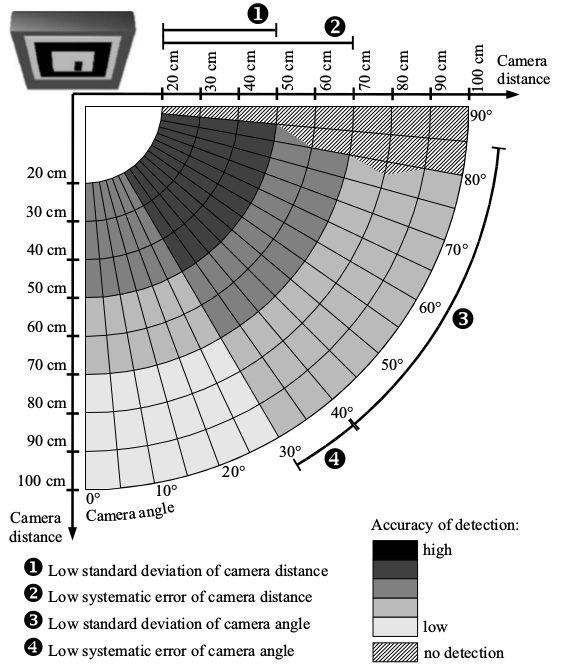
\includegraphics[scale=0.5]{./fig/acc_func.png}
\caption{Accuracy as a function of camera
distance and relative camera angle\cite{abawi2004accuracy}}
\label{fig:acc_func}
\end{figure}

Another research "Analysis of Tracing Accuracy for Single-Camera Square-Marker-Based Tracking"\cite{pentenrieder2006analysis} also presented a tracking accuracy analysis based on simulated ground truth data. Their accuracy evaluation of the visual marker based tracking system are based on the error and standard deviation. Their study only looks at the corner detection error but not consider pose estimation errors. Their experimental design follows "one-factor-at-a-time" principle and then also consider the combinations of all input factors. I also learned from this idea, which means firstly I studied the influence of \textbf{height}(distance of the marker) and \textbf{angle}(viewing angles) separately, after that I studied the combination of these influenced factors which means \textbf{height} and \textbf{angle} would be considered at the same time. They provided the following results:

\begin{itemize}
\item For larger distances the translational pose error and rotational pose error both increase. 
\item When the camera and marker form a certain small angle, it gets the smallest translational pose error and rotational pose error. But if the angle too small or the camera gradually becomes vertical to the marker, the translational pose error and rotational pose error would get bigger.
\end{itemize}

These results are shown in figure \ref{fig:Error_distance_angle} which are actually similar to the results in \cite{abawi2004accuracy}, but just in different form to represent it.

We can find that both researches \cite{abawi2004accuracy} and \cite{pentenrieder2006analysis}
were based on experimental data to describe the tracking accuracy, but they actually did not provide a "traditional function" to describe the accuracy, just like this simple form $f(x,y,z) = ax+by+cz$, where \texttt{f} is the desired accuracy function, \texttt{x}, \texttt{y}, \texttt{z} are the possible influencing factors of the accuracy function. 

\begin{figure}[H]
\centering
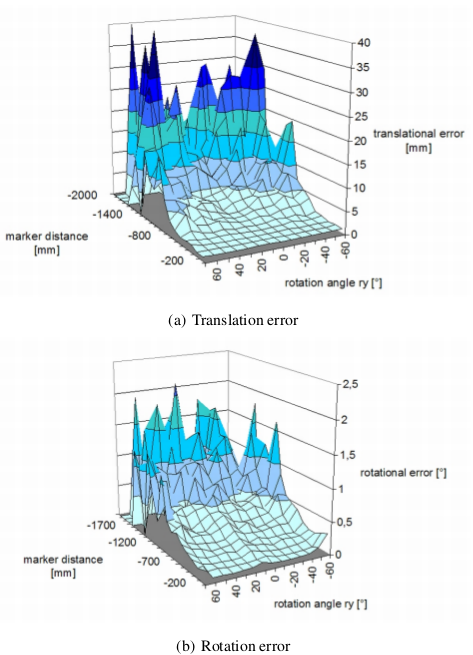
\includegraphics[scale=0.7]{./fig/Error_distance_angle.png}
\caption{Error for camera distance and rotation angle\cite{pentenrieder2006analysis}}
\label{fig:Error_distance_angle}
\end{figure}

\subsection{The desired accuracy function}
To fill this gap in this field, in our project we created the real "accuracy function", which means in the detection area of the given marker and camera, if one position coordinate is given we can obtain the information of accuracy at this corresponding position from the "accuracy function".

\begin{figure}[H]
\centering
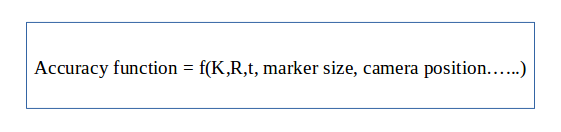
\includegraphics[scale=0.8]{./fig/acc_simple.png}
\caption{One simple example for the form of accuracy function, the influencing factors could be the camera intrinsic parameters; camera extrinsic parameters; the size of planar marker; the position of camera and so on}
\label{fig:acc_simple}
\end{figure}
%------------------------------------------
In this project we proposed the assumption that the condition number distribution can be interpreted as our desired accuracy function. 

Firstly, we convert the selected grid-based rectangle region which contains the detection region of the marker into a $m \times n$ matrix. This process is shown in figure \ref{fig:mncells}.

\begin{figure}[H]
\centering
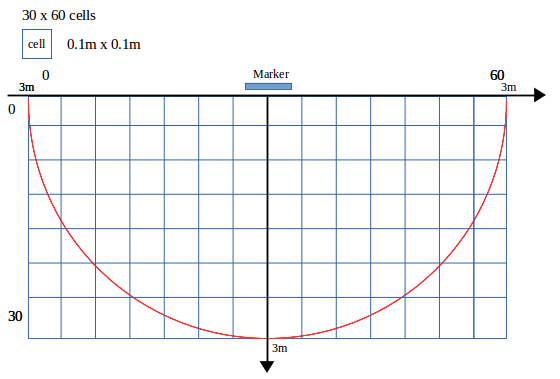
\includegraphics[scale=0.8]{./fig/mncells.png}
\caption{The detection region of the marker is defined as a semicircle with radius 3 meter, the $3m \times 6m$ rectangle region is grid-based and each cell is $0.1m \times 0.1m$, this region would be converted into a $30 \times 60$ matrix.}  
\label{fig:mncells}
\end{figure}

For each grid-cell there maybe several camera poses locate on it. Then we compute the average value \texttt{c} of all condition numbers of these camera poses fall onto the same cell, this average value \texttt{c} can be treated as the condition number of this cell. This process is shown in figure \ref{fig:cell_cn}.

\begin{figure}[H]
\centering
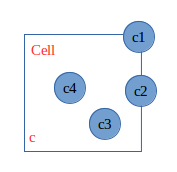
\includegraphics[scale=0.8]{./fig/cell_cn.png}
\caption{The blue square represents one cell and each blue circle represents one camera position. Condition number of this cell: $c = mean(c_1 + c_2 +c_3 + c_4)$}  
\label{fig:cell_cn}
\end{figure}

After that we can get a similar condition number distribution like the matrix shown in figure \ref{fig:conditionNum_mat}.
\begin{figure}[H]
\centering
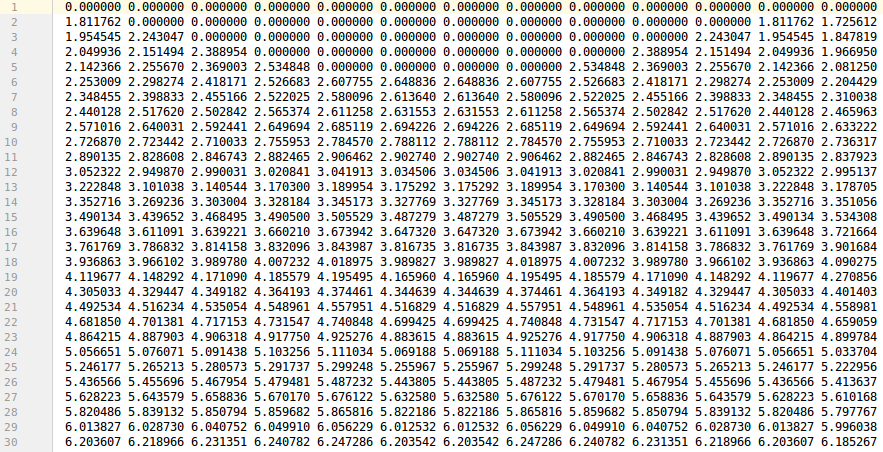
\includegraphics[scale=0.5]{./fig/conditionNum_mat.png}
\caption{An simple example of condition number distribution matrix, which is a $30 \times 60$ matrix, the above only shows part of the condition number distribution matrix}  
\label{fig:conditionNum_mat}
\end{figure}

After that if we want, we can divide the condition numbers into several degrees between the maximum and minimum, treating them as accuracy distribution. Finally, we can get the accuracy degree at given camera position. This whole precess is shown in figure \ref{fig:mc_process}.

\begin{figure}[H]
\hspace*{3cm}
\centering
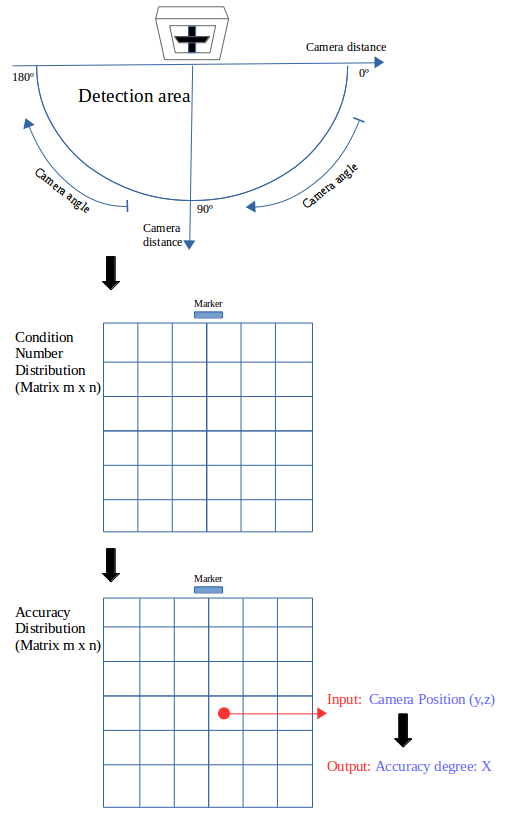
\includegraphics[scale=0.8]{./fig/mc_process.png}
\caption{Process...TODO}  
\label{fig:mc_process}
\end{figure}

From this we can find that the accuracy distribution(accuracy function) is affected by camera intrinsic, extrinsic parameters, the size of marker and the camera pose. And the key to find the accuracy function is : \texttt{Find out the condition number distribution.} 

Also the condition number distribution was used for our motion planning algorithms in chapter \ref{chap:Motion_planning}. In the following sections I will explain detailedly why the condition number distribution can be interpreted as the accuracy function and how we can get the condition number distribution in our simulations.

\subsection{Homography estimation}
\textbf{What is a homography?} 

A 2D point $(x,y)$ in the image plane can be represented as $(x_i,y_i,z_i)$ in 3D plane, where $x = \frac{x_i}{z_i}$ and $y = \frac{y_i}{z_i}$. This process is called homogeneous
representation of a 2D point. And the \textbf{homography matrix} is a non-singular $3 \times 3$ matrix which describes the linear mapping relationship between two planes in 2D homogenous coordinates(usually describes the transformation of some points in the common plane between two images, shown in figure \ref{fig:homo_es}). 

\begin{figure}[h]
\centering
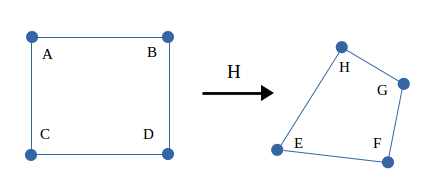
\includegraphics[scale=0.5]{./fig/homo_es.png}
\caption{Homography matrix}  
\label{fig:homo_es}
\end{figure}

We assume that there is a pair of matched feature points $p_1$ and $p_2$ in two different planes. Directly we can use homography matrix to describe the transformation between $p_1$ and $p_2$:
\begin{align*}
 p_2 = Hp_1  
\end{align*}
\begin{align*}
\begin{bmatrix} u_2 \\ v_2 \\ 1  \end{bmatrix}
=
\begin{bmatrix} h_1 & h_2 & h_3 \\
                h_4 & h_5 & h_6 \\
                h_7 & h_8 & h_9 \end{bmatrix}
\begin{bmatrix} u_1 \\ v_1 \\ 1  \end{bmatrix}
\end{align*}
where \textbf{H} is the homography matrix. We set $h_9 = 1$ and then reform the above formula:
\begin{align*}
h_1u_1 + h_2v_1 + h_3 - h_7u_1u_2 - h_8v_1u_2 &= u_2 \\
h_4u_1 + h_5v_1 + h_6 - h_7u_1v_2 - h_8v_1v_2 &= v_2 
\end{align*}

From above equations we find that there are now 8 unknowns($h_1 \sim h_8$) existed in 2 equations. In order to solve \texttt{H} we still need additional six equations, which means we need totally 4 pairs of points.

The Direct Linear Transform(DLT) is a common standard algorithm used
to solve for the homography matrix \texttt{H} given a sufficient set of corresponding point.
We notice that \texttt{H} can be changed by multiplying by an arbitrary
non-zero constant without altering the projective transformation. So usually $h_9$ should be set as $h_9 = 1$. In this case a homogeneous matrix only has 8 degrees of freedom even
though it contains 9 elements, which means we only need to solve these 8 unknown variables. From above equation we know that each pair of matched points can build one constrain for DLT. So we need 4 pairs of matched points to solve homography matrix \texttt{H}. And in our project the detected marker has 4 corner points for estimating of homography.
After estimating the homography we can get our expected rotation matrix \textbf{R} and translation vector \textbf{t} from corresponding homography matrix \textbf{H}.

\texttt{Normalizing transformations:}

For DLT algorithm the normalization of the measurements is a important step to improve the quality of the estimated homography. Normalization of the data consists of translation and scaling of image coordinates. This normalization should be carried out before applying the DLT algorithm.

Recall that the DLT formula \ref{equ:dlt} for 6 pairs of points, we can derive a similar formula for 4 pairs of points:
\begin{align}\label{equ:ah4}
 Ah = \begin{bmatrix} P_1^T & 0 & -u_1P_1^T\\
                 0 & P_1^T & -v_1P_1^T\\
                 \vdots & \vdots & \vdots\\
                 P_4^T & 0 & -u_4P_4^T\\
                 0 & P_4^T & -u_4P_4^T\\ \end{bmatrix} 
 \begin{bmatrix} t_1 \\ t_2 \\ t_3 \\ t_4 \\
                 t_5 \\ t_6 \\ t_7 \\ t_8 \\ \end{bmatrix} 
 = 0.         
\end{align}
The normalization is basically a preconditioning to decrease condition number of the matrix A(when there is noise in the measurement data, the more severe the change in the condition number, the more sensitive the method is to errors, and the less robust the method is. So low condition number of matrix \texttt{A} for our simulation is desired).
And it is already proven that the DLT algorithm is in practice invariant to similarity transformations\cite{hartley2000multiple}.

"Apart from improved accuracy of results, data normalization provides a second desirable benefit, namely that an algorithm that incorporates an initial data normalization step will be invariant with respect to arbitrary choices of the scale and coordinate origin. This is because the normalization step undoes the effect of coordinate changes, by effectively choosing a canonical coordinate frame for the measurement data.\cite{hartley2000multiple}"

For our case we also used the \texttt{isotropic scaling.} method which is also mentioned in \cite{hartley2000multiple}.
We can summarize the steps of isotropic scaling as follows:
\begin{enumerate}
\item The four image points(also the four object points) are translated so that their centroid is at the origin.
\item Then the four points are scaled so that the mean distance from the origin is $ \sqrt{2}$.
\end{enumerate}

This process is shown in figure \ref{fig:normalization}.
\begin{figure}[h]
\centering
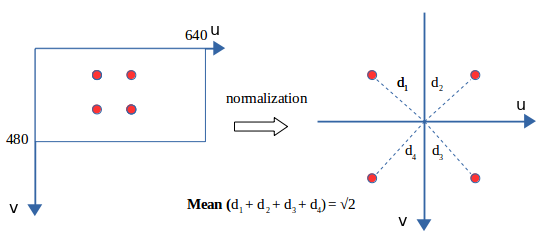
\includegraphics[scale=0.8]{./fig/normalization.png}
\caption{Normalization of 4 image points, this process can reduce condition number of matrix \texttt{A} and maximize the robustness of the DLT
homography estimation against noise}  
\label{fig:normalization}
\end{figure}

\texttt{Why is normalization essential?} %TODO

There is already a complete good answer in \cite{hartley2000multiple}. All in all we apply normalization is in order to set all entries in matrix \texttt{A} have similar magnitude and increase the robustness of accuracy function.

However, the normalization still has some disadvantages:
\begin{itemize}
\item The estimated homography depends on the similarity transforms.
\item The normalization matrices are computed from
noisy pixel measurements, and therefore sensitive to outliers.
\end{itemize}

To overcome these disadvantages a (non-iterative)method for estimating homographies does not
rely on coordinate normalization is proposed in \cite{rangarajan2009estimating} which is by avoiding normalization and instead using a \texttt{Taubin estimator}, that is unaffected by similarity transformations of the correspondences in the two views. 

In our project we will compare the results of the accuracy function for estimating homographies without normalization and with normalization.

\subsection{Connect accuracy function with condition number}
In this section I will explain why the condition number distribution can be interpreted as the accuracy function.\\

\texttt{Planar Point Configuration for Pose Estimation:}

In previous section we already introduced the pinhole camera model and the pose estimation from 3D points. And in our project we applied a planar marker to estimate the camera pose. Specially if the control points are all on a plane, we can reduce the degree of freedom of the rotational matrix \texttt{R}.(Now we can use two angles instead of three angles to represent rotational matrix \texttt{R}:
\begin{align*}
\Aboxed{R = [r_1, r_2, r_3] \to R = [r_1, r_2]}
\end{align*}
Because all control points are located on a plane, we can define a 2D subspace instead of three-dimensional coordinates in 3D world, set the Z-coordinate as 0:
\begin{align*}
X_i^W = \begin{bmatrix} X_i^W \\ Y_i^W \\ Z_i^W \end{bmatrix} \implies 
X_i^W = \begin{bmatrix} X_i^W \\ Y_i^W \\ 0 \end{bmatrix}
\end{align*}
Under the perspective projection model, through the projection matrix \texttt{P} mapping three-dimensional space points \texttt{X} onto \texttt{u} on the image plane. The transformation can be represented as following equation:  
\begin{align*}
s\overline{u} &= P\overline{X} \\
s \begin{bmatrix} u \\ v \\ 1 \end{bmatrix} &= P \begin{bmatrix} X^W \\ Y^W \\ Z^W \\ 1 \end{bmatrix} = \begin{bmatrix} p_1 & p_2 & p_3 & p_4 \end{bmatrix} \begin{bmatrix} X^W \\ Y^W \\ Z^W \\ 1 \end{bmatrix}
\end{align*}
where $\overline{u} = \begin{bmatrix} u,&v,&1 \end{bmatrix}$, $\overline{X}=\begin{bmatrix} X^W, &Y^W, &Z^W, &1 \end{bmatrix}$ are represented as homogeneous coordinates and \texttt{s} is the non-zero scale factor. We assume that plane $\pi$ is the plane where our fiducial marker are located(plane $\pi$ is the \texttt{XOY} plane of the object coordinate system). For points on the plane $\pi$, there is $Z_i = 0$, then we can get following deformation:
\begin{align*}
s \begin{bmatrix} u \\ v \\ 1 \end{bmatrix} &= P \begin{bmatrix} X^W \\ Y^W \\ 0 \\ 1 \end{bmatrix} = 
\underbrace{\begin{bmatrix} p_1 & p_2 & p_3 \end{bmatrix}}_\text{H}
 \begin{bmatrix} X^W \\ Y^W \\ 1 \end{bmatrix}
\end{align*}
where $H = \begin{bmatrix} p_1,&p_2,&p_3 \end{bmatrix}$, we can describe $\overline{X_{\pi}}$ as $\overline{X_{\pi}} = \begin{bmatrix} X^W,&Y^W,&1 \end{bmatrix}$, then we get following equation:
\begin{align}\label{equ:suhx}
s\overline{u} &= H\overline{X_{\pi}}
\end{align}

Similar to 6 pairs of points DLT algorithm derivation in previous section and in our project we used a fiducial marker with four control points(any 3 points are not collinear) on a plane. Solving equation \ref{equ:suhx} is equal to solve the following equation, which has the similar form as formula \ref{equ:ah4}:
\begin{align*}
\Aboxed{Ah = 0}
\end{align*}
\begin{align*}
A =
\begin{bmatrix} 0 & 0 & 0 & -X_1 & -Y_1 & -1 & v_1 X_1 & v_1 Y_1 & v_1 \\
                X_1 & Y_1 & 1 & 0 & 0 & 0 & -u_1 X_1 & -u_1 Y_1 & -u_1 \\
                0 & 0 & 0 & -X_2 & -Y_2 & -1 & v_2 X_2 & v_2 Y_2 & v_2 \\
                X_2 & Y_2 & 1 & 0 & 0 & 0 & -u_2 X_2 & -u_2 Y_2 & -u_2 \\
                0 & 0 & 0 & -X_3 & -Y_3 & -1 & v_3 X_3 & v_3 Y_3 & v_3 \\
                X_3 & Y_3 & 1 & 0 & 0 & 0 & -u_3 X_3 & -u_3 Y_3 & -u_3 \\
                0 & 0 & 0 & -X_4 & -Y_4 & -1 & v_4 X_4 & v_4 Y_4 & v_4 \\
                X_4 & Y_4 & 1 & 0 & 0 & 0 & -u_4 X_4 & -u_4 Y_4 & -u_4 \\
\end{bmatrix}
\end{align*}

where $A \in \mathbb{R}^{8 \times 9}$ and $h = \begin{bmatrix}
r_1^T,&r_2^T,&t^T
\end{bmatrix}^T \in  \mathbb{R}^9$.
Under additional constraint $ \norm{h} = 1$, \texttt{h} is the homography matrix with 8 unknowns.

However in the actual situation we set noisy(Gaussian distribution) for each image points, again assuming noisy measurements for image points $\widetilde{u_i} = u_i + \xi_i$, we get the matrix $\widetilde{A} = A + E$ with noise. Due to the presence of noise, in the most cases $\widetilde{A} h \neq 0$, so \texttt{h} would be estimated by minimization of $\widetilde{A} h$, due to $Ah = 0$,  this problem can be solved also by minimization of $\norm{Eh}_2^2$:
\begin{align}\label{equ:aheh}
h = argmin_h \norm{\widetilde{A}h}_2^2 = argmin_h \norm{Eh}_2^2,\quad with  \quad \norm{h} = 1
\end{align}

Solving equation \ref{equ:aheh} is actually equivalent to apply a singular value decomposition(SVD) of $\widetilde{A} = \widetilde{U}\widetilde{S}\widetilde{V}$ for this DLT algorithm, where the solution of equation \ref{equ:aheh} is $ h = \widetilde{v_9}$ with $\widetilde{v_9}$ being the right singular vector of $\widetilde{A}$, associated with the least singular value $\widetilde{s_9}$.

\begin{figure}[H]
\centering
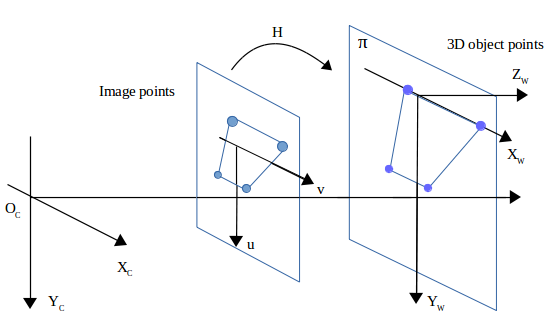
\includegraphics[scale=0.5]{./fig/H.png}
\caption{The perspective projection of the 3D plane}  
\label{fig:H}
\end{figure}

\texttt{Why is condition Number?}
 
For the linear problem, the condition number of the measurement matrix is an important factor affecting its numerical stability.

If the singular values of matrix \textit{A} are $d_1,d_2,\dotsm ,d_9(d_1 \geq d_2 \dotsm \geq d_9 = 0)$, then the condition number of matrix \textit{A} is:
\begin{align*}
c(A) = \frac{d_1}{d_8}
\end{align*}

In previous researches from \cite{abawi2004accuracy} and \cite{pentenrieder2006analysis} they described the accuracy function with the rotational error and translational error. And in \cite{dynamic_markers} there is a interesting results, when the rotational error and translational error decrease or increase, the condition number at corresponding position also becomes smaller or bigger. They have a similar trend in terms of different camera pose. Through this discovery we therefore made our assumption that we can use condition number to describe the accuracy function. And through our simulations we already verified this assumption.

In following sections I will explain how our simulations were performed.

\section{Simulation design}
\subsection{Simulation frame setup}

For the simulation the two most important objects are: \texttt{marker} and \texttt{camera}. 
In order to make simulation between marker and camera, we need to set some properties of both.
\subsubsection{Marker}
We used a square fiducial marker for camera pose estimation. More precisely the four vertices of the square marker are defined as the control points, which are then needed to project onto the camera image. Because in \cite{dynamic_markers} it was already verified that for 4 points in most cases the vertices of a square marker are the optimal control points, therefore these four vertices are represented as our detected features for camera.

We set that the center of the marker is the origin of world coordinate system($O-X_W Y_W Z_W$). And the fiducial planar marker was located on \texttt{XOY} plane in the world coordinate system. The positive direction of Z-axis points to the region where the cameras should be located on. The coordinates of the four control points under world coordinate system are:
\begin{enumerate}
\item Point 1: $(0.15,0.15)$
\item Point 2: $(0.15,-0.15)$
\item Point 3: $(-0.15,-0.15)$
\item Point 4: $(-0.15,0.15)$
\end{enumerate}
In the simulation the default size of the marker was set as $0.3m \times 0.3m$ and we set the marker as fixed at the origin of the coordinate system, of course we can change different size of the marker to fit more testing scenarios. 

The simulation scene of the planar marker is illustrated in figure \ref{fig:marker}.
\begin{figure}[H]
\centering
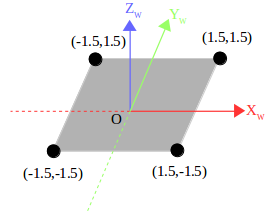
\includegraphics[scale=0.5]{./fig/marker.png}
\caption{A marker with size $0.3m \times 0.3m$, four features at each corner.}  
\label{fig:marker}
\end{figure}

  
\subsubsection{Camera}
We already introduce the camera model in previous section and it is well-known that we often use 
$\begin{bmatrix}
u & v & 1
\end{bmatrix}^T$ to represent the position of a 2D point in pixel coordinates, corresponding 
$\begin{bmatrix}
X_W & Y_W & Z_W & 1
\end{bmatrix}^T$ is used to represent the position of 3D point in world coordinate system. According to the pinhole camera model, we know the following projective mapping from world coordinate system to pixel coordinate system:
\begin{equation}
Z_C \begin{bmatrix} u \\ v \\ 1 \end{bmatrix}
      = K 
        \begin{bmatrix} R | t \end{bmatrix}                                          
        \begin{bmatrix} X_W \\ Y_W \\ Z_W \\ 1 \end{bmatrix}
\end{equation}
where \textit{K} is the intrinsic parameters and we set it's default value as
$\mathbf{K} = \begin{bmatrix} 800 & 0 & 0\\
                 0 & 800 & 240\\
                 0 & 0 &1\end{bmatrix}$, the extrinsic parameters \texttt{R} and \texttt{t} are the variables we are interested in. By setting different camera positions in our simulation we obtain different camera pose, that is the rotation matrix \texttt{R} and translation vector \texttt{t}. It is worth noting that in our project we did not consider the camera distortion problem for now. 

We set the image default size as $\mathit{640 \times 480[pixel^2]}$, through derivation of camera intrinsic parameters \texttt{K} in previous section we can easily find that parts of \texttt{K} parameters are related to the height and width of the image. Therefore if we change the size of the image, we also need to change the camera intrinsic parameters \texttt{K} correspondingly.   
 
Although we do not need to consider the camera distortion problem, in the real environment camera noise is an unavoidable factor. In order to simulate the reality of camera we set the image noise manually. For each image point we added a 2-dimensional Gaussian distribution:
\begin{python}
    def addnoise_imagePoints(self, imagePoints, mean = 0, sd = 2):
        """ Add Gaussian noise to image points
        imagePoints: 3xn points in homogeneous pixel coordinates
        mean: zero mean
        sd: pixels of standard deviation
        """
        imagePoints = np.copy(imagePoints)
        if sd > 0:
            gaussian_noise = np.random.normal(mean,sd,(2,imagePoints.shape[1]))
            imagePoints[:2,:] = imagePoints[:2,:] + gaussian_noise
        return imagePoints
\end{python}

\texttt{camera distribution:}\\
Normally each camera has a fixed detection range, in our simulation we fixed the position of planar marker, in this way we can image that each marker has a detection area just like the camera. Therefore the cameras can be treated as moved in the detection region of the marker. This idea is shown in figure \ref{fig:cm_invert}.
\begin{figure}[H]
\centering
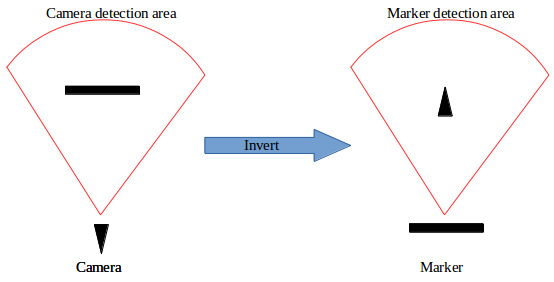
\includegraphics[scale=0.7]{./fig/cm_invert.png}
\caption{Invert camera and marker}  
\label{fig:cm_invert}
\end{figure}

Because in our situation the robot moves only on \textbf{YZ}-plane of world coordinates and the heights of the canter of the marker and camera lens always keep at the same level, this scenario is shown in figure \ref{fig:marker_camera}. Therefore we can simplify the 3D camera distribution shown in figure \ref{fig:cam3D2D}(a) into the 2D camera distribution shown in figure \ref{fig:cam3D2D}(b). 

\begin{figure}[H]
\centering
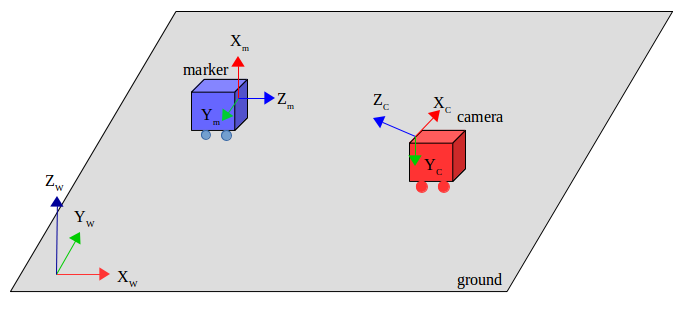
\includegraphics[scale=0.45]{./fig/marker_camera.png}
\caption{Two-robot Caterpillar}  
\label{fig:marker_camera}
\end{figure}

\begin{figure}[H]
  \centering
  \begin{subfigure}[b]{0.8\linewidth}
    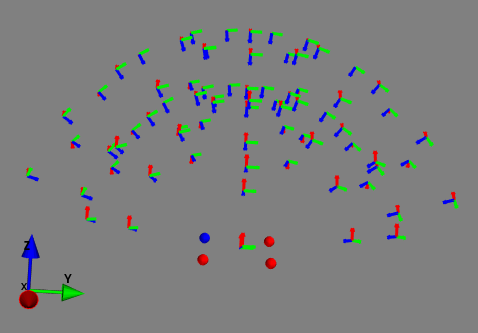
\includegraphics[width=\linewidth]{./fig/cam3D.png}
    \caption{An Example for camera distribution in 3D. The camera are distributed evenly on spheres of different radius. Each camera(positive direction of Z-axis) should look at the origin of the plane.}
  \end{subfigure}
  \begin{subfigure}[b]{0.8\linewidth}
    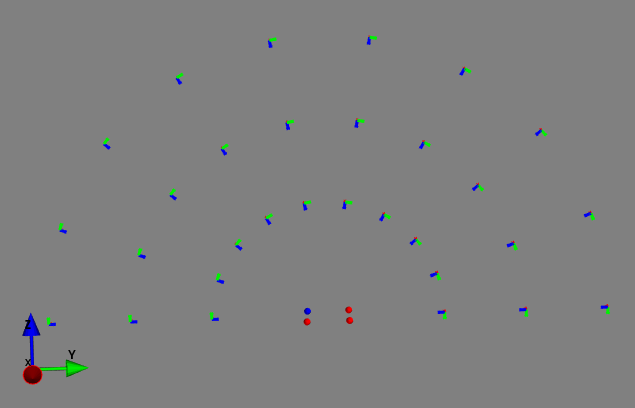
\includegraphics[width=\linewidth]{./fig/cam2D.png}
    \caption{An Example for camera distribution in 2D. The camera are distributed evenly on YZ-plane. Each camera(positive direction of Z-axis) should look at the origin of the plane. We apply this 2D case in our simulation.}
  \end{subfigure}
  \caption{Camera distribution}
  \label{fig:cam3D2D}
\end{figure}

In our simulation we set a very important rule:

\texttt{Each camera should look at the center of the planar marker!}

\subsection{Simulation approach}

A very common approach for simulations or experiments is the "one-factor-at-a-time" method\cite{wiki_ofaatm}, which means we should study only one affected factor while all others are kept constant. But this approach fails to consider the effect of multiple variable combinations on one system or on one function. So beyond this approach we also need to consider the combinations of all inputs. For example in our simulation we need to consider not only the influence of height and angle separately but also the interactions of height and angle.

Therefore we applied "one-factor-at-a-time" method at the beginning of the simulation, trying to find out some rules or clues for accuracy function, we can treat it as heuristics. On the basis of that we estimated interactions between different factors and trying to find out the final experimental conclusion from our simulation.

In our simulation we studied two important factors:
\begin{itemize}
\item \texttt{Height}: the distance between camera and marker, we can also call it \texttt{radius}. 
\item \texttt{Angle}: the angle between Z-axis of camera and marker plane.
\end{itemize}
\section{Results}
We have already pointed out that the condition number distribution can be interpreted as the accuracy function and later the condition number distribution can be used in our pathfinding. Therefore in this section we provide the results all about condition number distribution. 

Also according to the research in \cite{pentenrieder2006analysis}, our desired results are:
\begin{itemize}
\item If the angle between camera and marker plane is fixed, the closer the distance between camera and marker, the smaller the condition number is.
\item If the distance between camera and marker is fixed, the smaller the angle between camera and marker plane, the smaller the condition number is.
\end{itemize}

In previous sections we already mentioned that how important the normalization of homography is. In this part different results without normalization and with normalization would be compared detailedly. Then Therefrom we found out the best solution which is satisfied our desired results.

In order to compute the condition number distribution the object points and image points were transformed like follows in four ways: 
\begin{enumerate}
\item object points: no normalized, image points: no normalized
\item object points: regular normalized, image points: regular normalized
\begin{python} 
scale = np.sqrt(2) / meandist # Translation and scaling 
\end{python}
\item object points: regular normalized, image points: normalized
\begin{python} 
scale = 1 # Only translation, no scaling 
\end{python}
\item object points: regular normalized, image points: normalized
\begin{python}
scale = radius*np.sqrt(2) / meandist 
\end{python}

\end{enumerate}

where in the second case the \texttt{regular normalized} means the four points are scaled so that the mean distance from the origin is $ \sqrt{2}$, for the third case the four image points are only translated but not scaling, for the fourth case the four image points are scaled so that the mean distance from the origin is $ radius * \sqrt{2}$(radius is the distance from camera to marker).

In order to represent the results clearly, we used colormap \texttt{magma} form \texttt{matplotlib} library\cite{matplotlib} to represent our data set:
\begin{itemize}
\item Dark color(black) $\to$ small condition number
\item Light color(yellow) $\to$ big condition number
\end{itemize}

\begin{figure}[H]
\centering
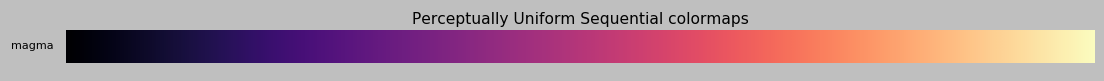
\includegraphics[scale=0.34]{./fig/magma.png}
\caption{Colormap \textit{magma} from \textit{matplotlib} library}  
\label{fig:magma}
\end{figure}
%======================================================================
\texttt{Condition number distribution without normalized homography:}

At first, we computed the condition number of each camera pose without normalization of the homography.

\begin{python}
# Compute the condition number without normalization
cond_num = gd.matrix_condition_number_autograd(*input_list, normalize = False)
\end{python} 

And we applied "one-factor-at-a-time" method that we made simulations for \texttt{angle} and \texttt{height} separately and we got the following results which are shown in figure \ref{fig:angle_height}: 

\begin{figure}[H]
  \centering
  \begin{subfigure}[b]{1.0\textwidth}
    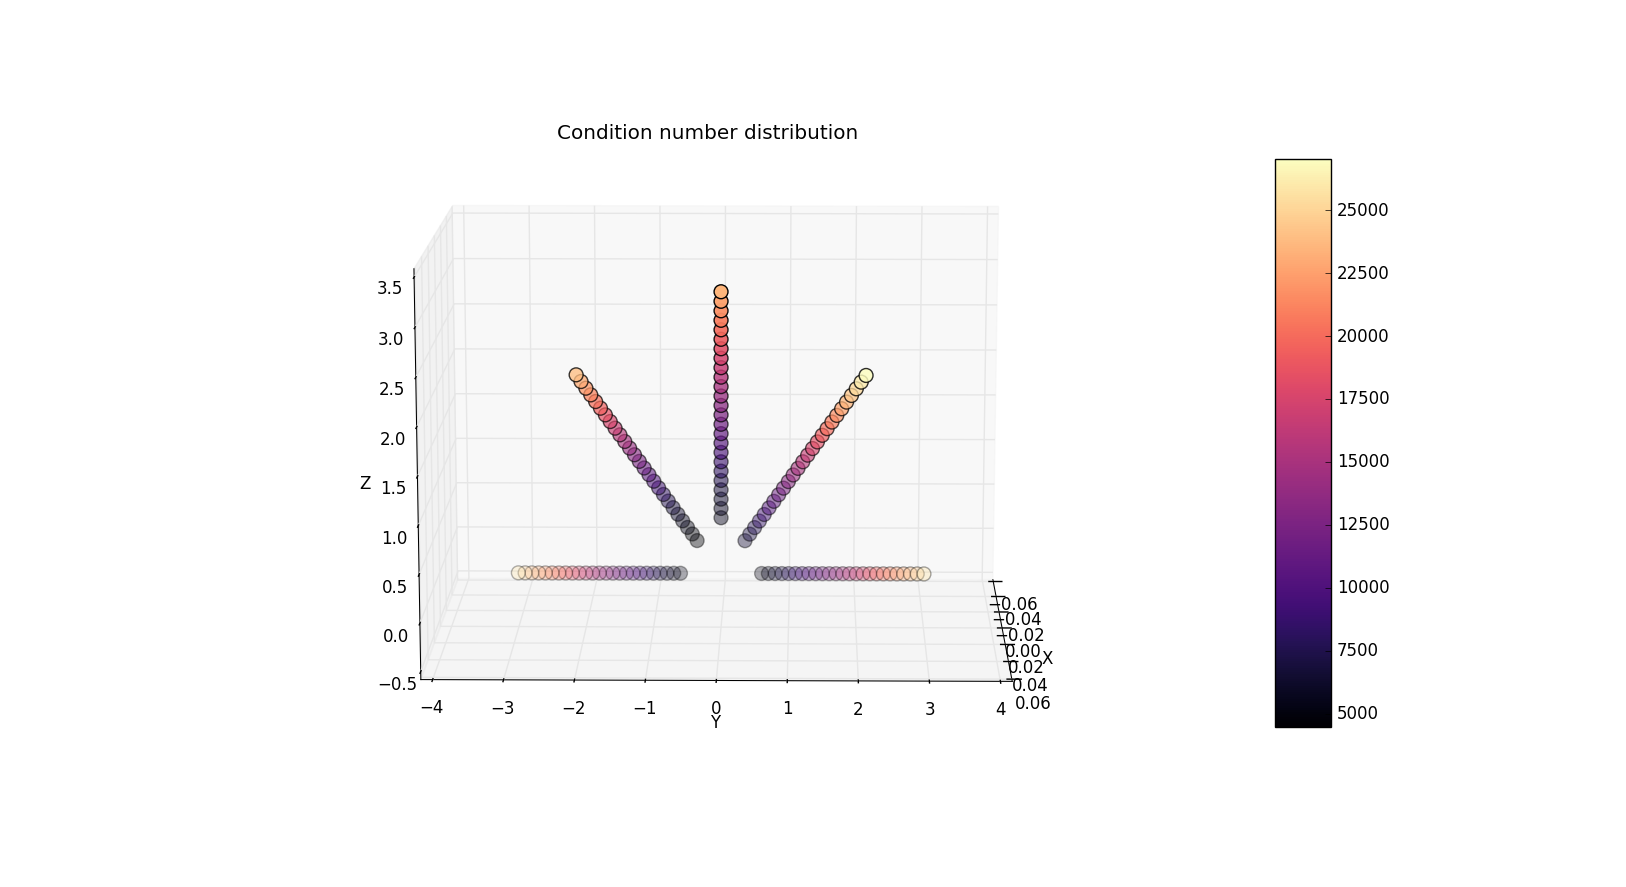
\includegraphics[width=\textwidth]{./fig/only_height.png}
    \caption{Influence of the height(distance between the cam1era and the marker) on the condition number of different camera positions while the angle is fixed as \SI{0}{\degree},\SI{45}{\degree},\SI{90}{\degree},\SI{135}{\degree} and \SI{180}{\degree}}
  \end{subfigure}
  \begin{subfigure}[b]{1.0\textwidth}
    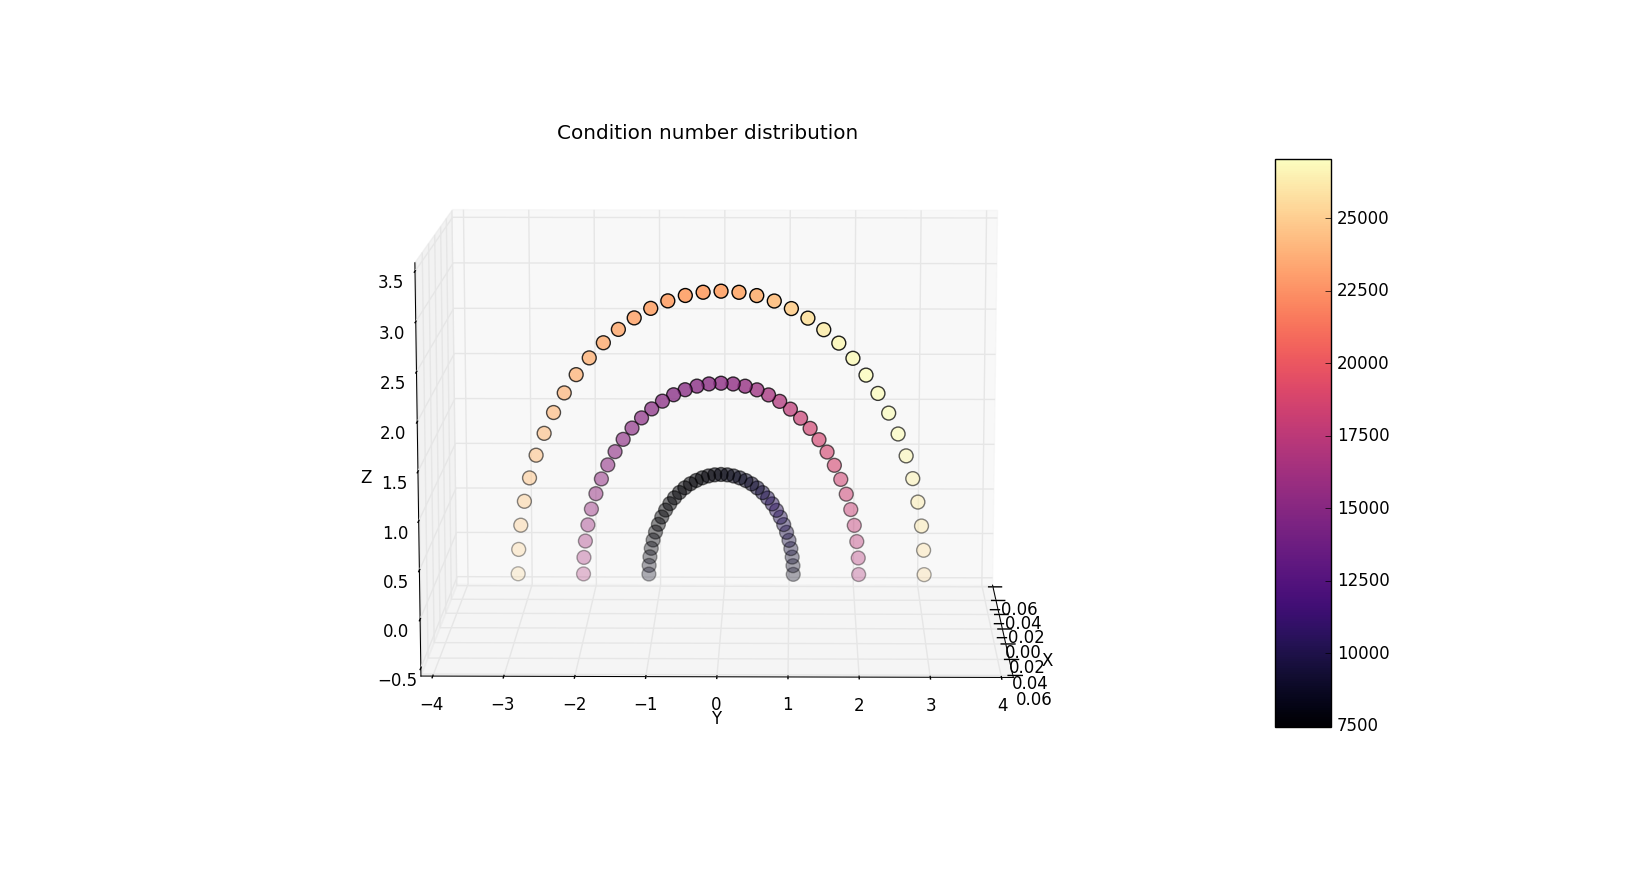
\includegraphics[width=\textwidth]{./fig/only_angle.png}
    \caption{Influence of the angle on the condition number of different camera positions while the height(distance between camera and marker) is fixed as 1.06666667m, 2.0333333 and 3m}
  \end{subfigure}
  \caption{Condition number distribution of different camera positions, each circle represents each camera position, different colors represent different values(figure \ref{fig:magma})}
  \label{fig:angle_height}
\end{figure}

\begin{figure}[H]
\hspace*{-4cm}
\centering
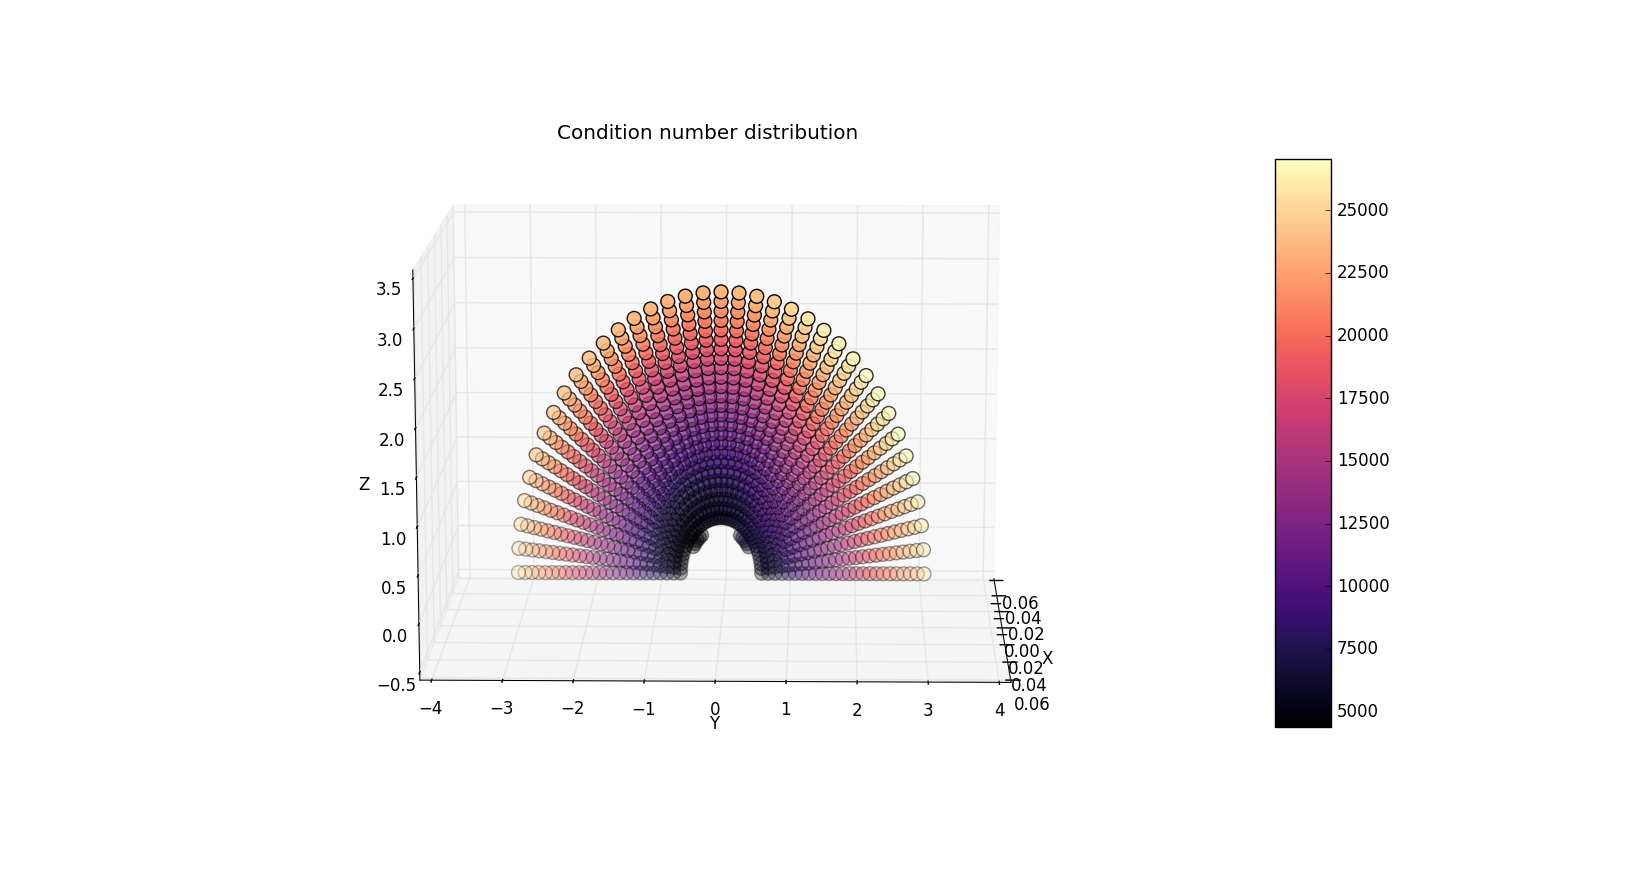
\includegraphics[scale=0.6]{./fig/cond_dis_noNor.png}
\caption{Condition number distribution(Interaction of \texttt{angle} and \texttt{height}), object points and image points are not normalized. The camera distribution is on YZ plane. The \texttt{angle} $\theta = [\SI{0}{\degree}, \SI{180}{\degree}]$, the step of angle is $\SI{5}{\degree}$, but in real world the angle can not be $\SI{0}{\degree}$ because of the constrain of DLT(three points that must be not collinear). The \texttt{height}(distance between camera and marker) as radius $ r= [0.1m, 3.0m]$, the step of radius is $0.1m$.}  
\label{fig:cond_dis_noNor}
\end{figure}

We can find that in figure \ref{fig:angle_height}(a) the condition number increases while the distance between camera and marker increases. This trend of condition number is consistent with previous results based on experiments in \cite{abawi2004accuracy} and \cite{pentenrieder2006analysis} and also is one of our desired result. 

However, in figure \ref{fig:angle_height}(b) it shows the condition number distribution is asymmetric. This is because that according to the equation mentioned in \cite{dynamic_markers}, we know that:
\begin{align*}
 c(A) = \norm{A}_2\norm{A^{-1}}_2 = \frac{s_{max}}{s_{min}}=\frac{s_1}{s_8}  
\end{align*}
and A is composed of four object points and four image points in our case,
we know that the object points are always set as constant(the coordinates in world coordinate system are fixed), so the only affected factor is related to the four image points. So we can see what is happened by image points:

Different camera position(Symmetrical cam position) on YZ plane has different rotation matrix \textbf{R}. And according to the corresponding rotation matrix \textbf{R} we can get different image points(camera model).

The symmetrical camera positions, which are closer to Z-axis ($\theta = 90$) and Y-axis ($\theta = 0$), get almost similar image points, similar image points lead to similar condition number. And the condition numbers on these symmetrical cam positions have smaller difference.
At somewhere $\theta$ between $0-90$, we get the biggest difference of condition number on symmetrical cam positions.

\begin{figure}[H]
\centering
\hspace*{-4cm}
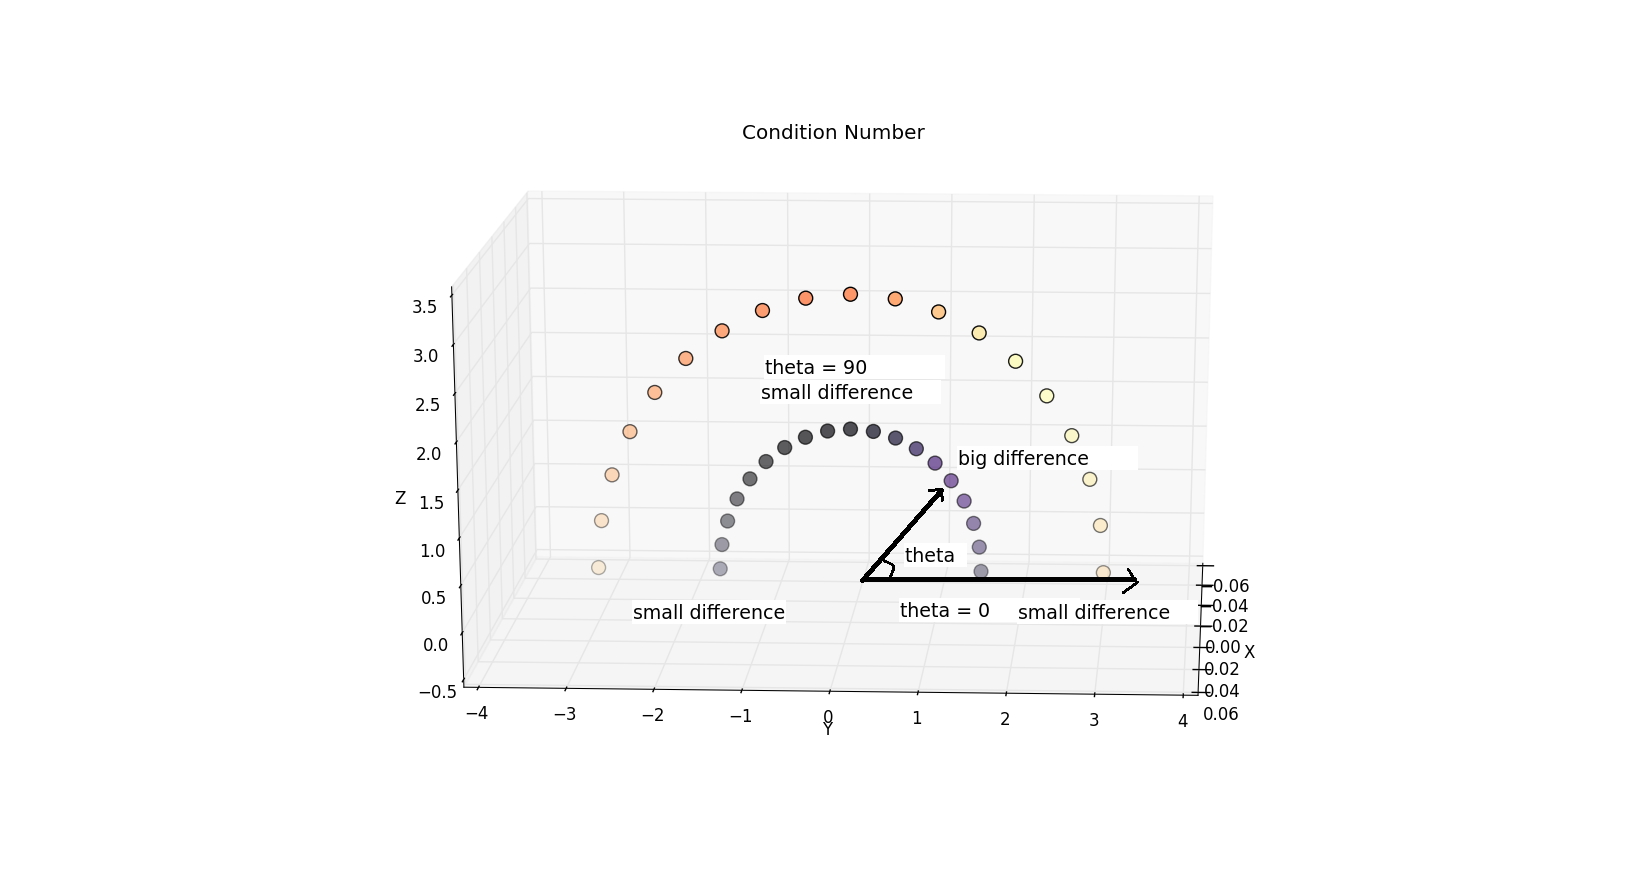
\includegraphics[scale=0.6]{./fig/connum_symm.png}
\caption{Symmetrical camera positions with different condition number}  
\label{fig:connum_symm}
\end{figure}

\begin{figure}[H]
  \centering
  \begin{subfigure}[b]{0.4\textwidth}
    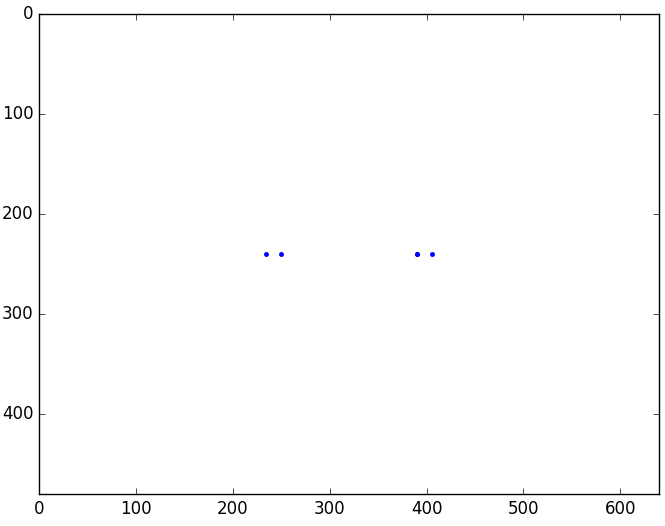
\includegraphics[width=\textwidth]{./fig/1.png}
    \caption{theta = $\SI{0}{\degree}$}
  \end{subfigure}
  \begin{subfigure}[b]{0.4\textwidth}
    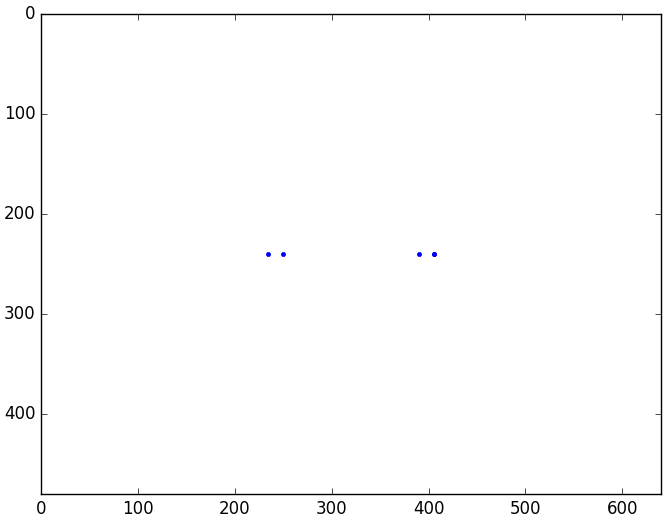
\includegraphics[width=\textwidth]{./fig/19.png}
    \caption{theta = $\SI{180}{\degree}$}
  \end{subfigure}
  
  \begin{subfigure}[b]{0.4\textwidth}
    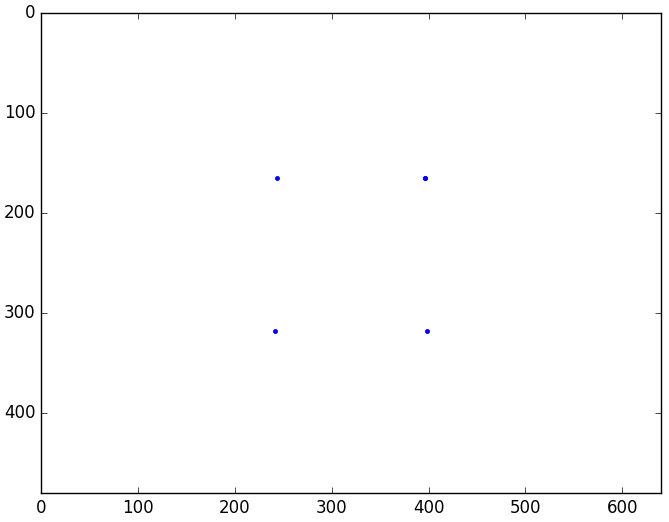
\includegraphics[width=\textwidth]{./fig/9.png}
    \caption{theta $\approx \SI{90}{\degree}, e.g. theta = \SI{89}{\degree}$}
  \end{subfigure}
  \begin{subfigure}[b]{0.4\textwidth}
    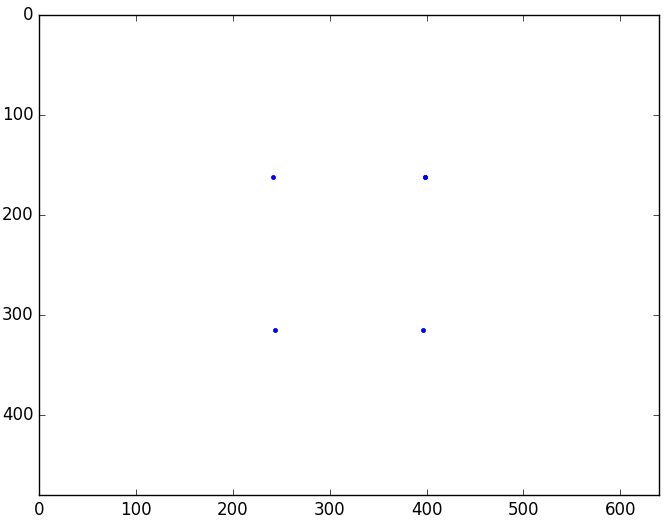
\includegraphics[width=\textwidth]{./fig/11.png}
    \caption{theta $\approx \SI{90}{\degree}, e.g. theta = \SI{91}{\degree}$}
  \end{subfigure}
    
    \begin{subfigure}[b]{0.4\textwidth}
    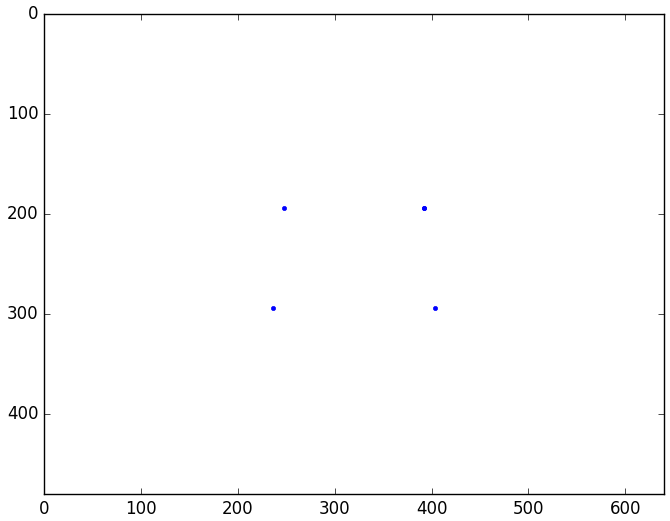
\includegraphics[width=\textwidth]{./fig/5.png}
    \caption{theta $\approx \SI{45}{\degree}$}
  \end{subfigure}
  \begin{subfigure}[b]{0.4\textwidth}
    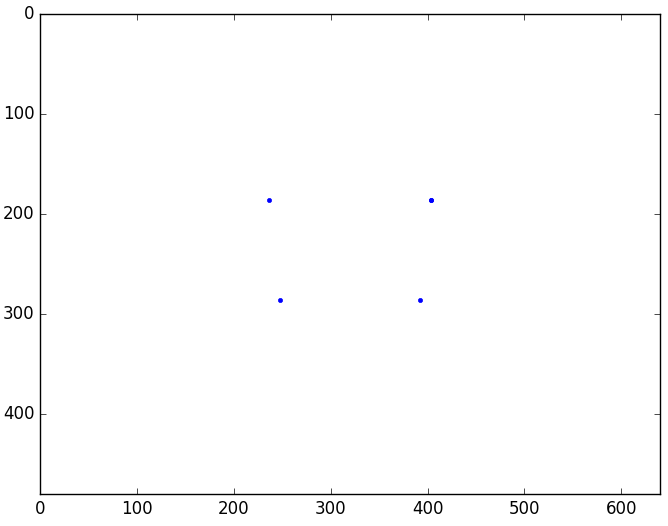
\includegraphics[width=\textwidth]{./fig/15.png}
    \caption{theta $\approx \SI{135}{\degree}$}
  \end{subfigure}
  \caption{When theta is equal to $\SI{0}{\degree}$ or $\SI{180}{\degree}$, image points exactly same. When theta closes to 90, image points exactly very similar. When theta closes to $\SI{45}{\degree}$ or $\SI{135}{\degree}$, image points have relative larger differences}
  \label{fig:119}
\end{figure}

In addition to asymmetric problem, there is another problem: 

The condition number is biggest when the angle of camera position is close to $\SI{90}{\degree}$, but this trend of condition number based on the change of angle is not a ideal and desired result. The reason for this problem is that without normalization of homography the differences of object points' order and image points' order are particularly large\cite{hartley2000multiple}. Therefore, we made regular normalization for both object points and image points in next step.\\

\texttt{Condition number distribution with normalized homography(regular normalization):}

We applied regular normalization for both object points and image points and made simulations under the same conditions as before.
 
\begin{python}\label{python:regular}
dist = []
pts = pts/pts[2, :]
for i in finiteind:
    c = np.mean(pts[0:2, i].T, axis=0).T
    newp1 = pts[0, i] - c[0]
    newp2 = pts[1, i] - c[1]
    dist.append(np.sqrt(newp1 ** 2 + newp2 ** 2))

dist = np.array(dist)
meandist = np.mean(dist)
scale = np.sqrt(2) / meandist # Translation and scaling
T = np.array([[scale, 0, -scale * c[0]], [0, scale, -scale * c[1]], [0, 0, 1]])
newpts = np.dot(T, pts)
return newpts,T
\end{python}

Figure \ref{fig:cond_dis_imageNor_angle_height} shows separately the condition number distribution in terms of \texttt{height} and \texttt{angle}, figure \ref{fig:cond_dis_imageNor} shows the condition number distribution at all positions.

\begin{figure}[H]
  \centering
  \begin{subfigure}[b]{1.0\textwidth}
    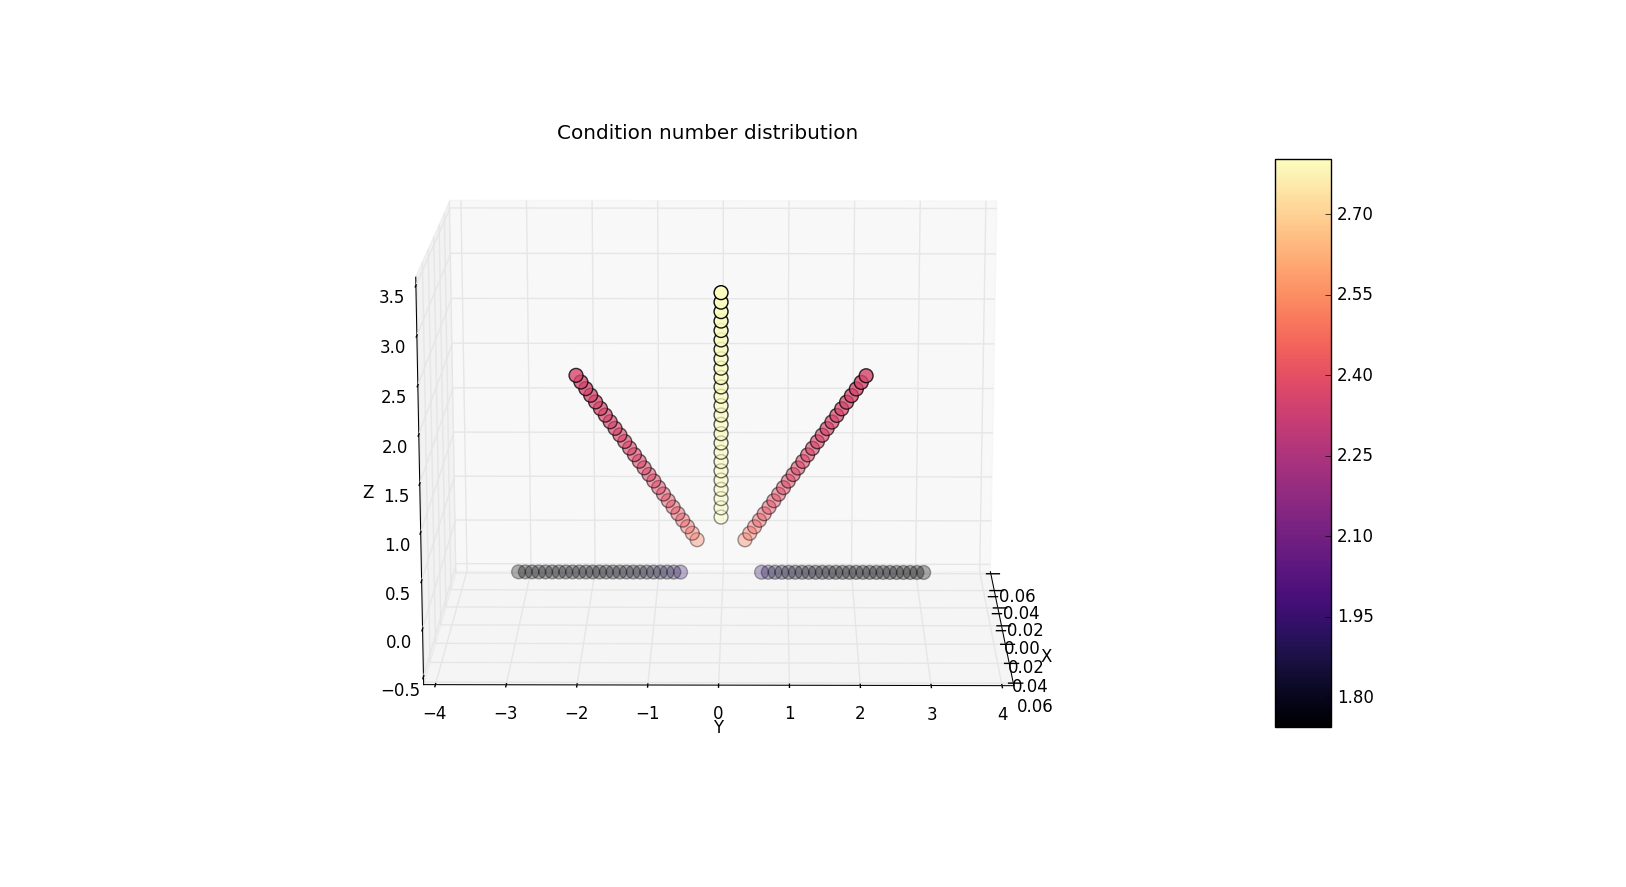
\includegraphics[width=\textwidth]{./fig/cond_dis_imageNor_height.png}
    \caption{Influence of the height(distance between the cam1era and the marker) on the condition number of different camera positions while the angle is fixed as \SI{0}{\degree},\SI{45}{\degree},\SI{90}{\degree},\SI{135}{\degree} and \SI{180}{\degree}}
  \end{subfigure}
  \begin{subfigure}[b]{1.0\textwidth}
    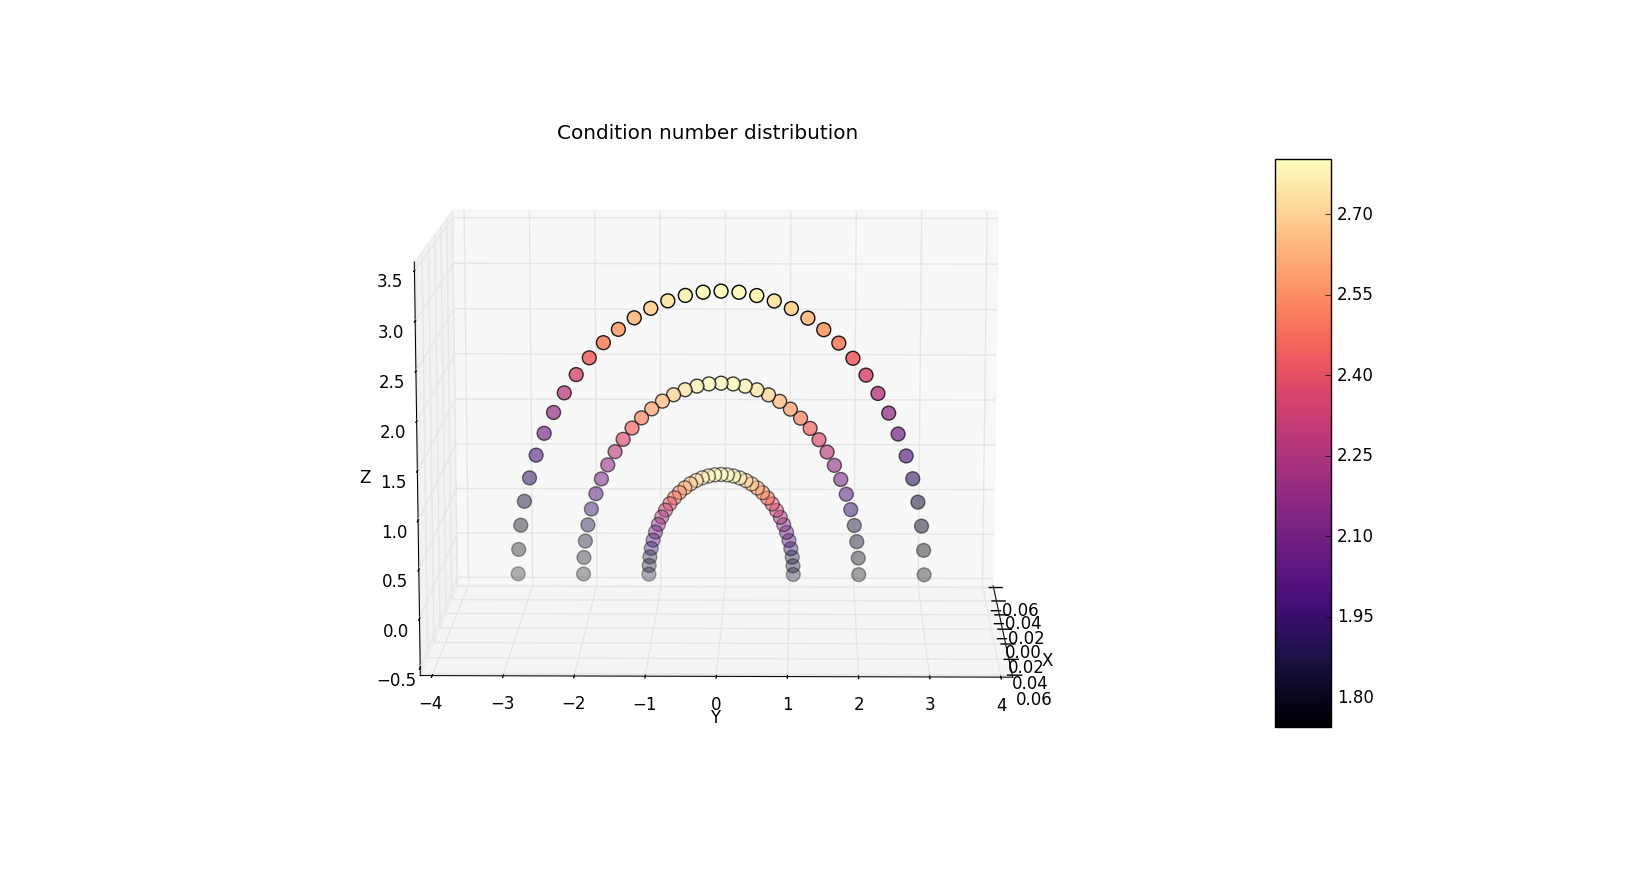
\includegraphics[width=\textwidth]{./fig/cond_dis_imageNor_angle.png}
    \caption{Influence of the angle on the condition number of different camera positions while the height(distance between camera and marker) is fixed as 1.06666667m, 2.0333333 and 3m}
  \end{subfigure}
  \caption{Condition number distribution of different camera positions, each circle represents each camera position, different colors represent different values(figure \ref{fig:magma})}
  \label{fig:cond_dis_imageNor_angle_height}
\end{figure}


\begin{figure}[H]
\hspace*{-4cm}
\centering
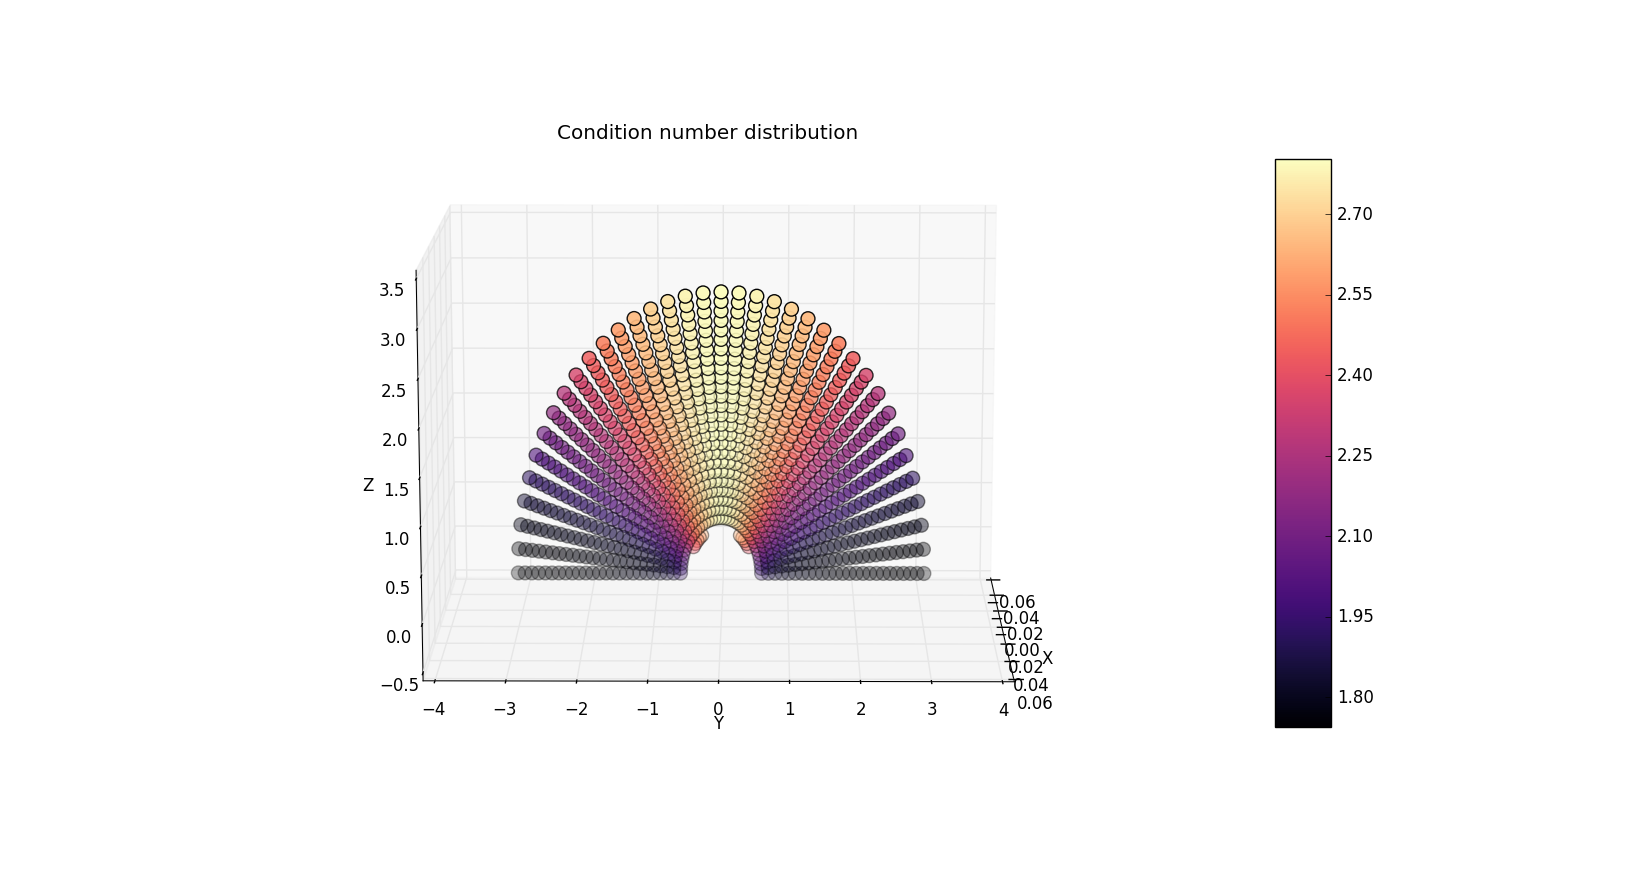
\includegraphics[scale=0.6]{./fig/cond_dis_imageNor.png}
\caption{Condition number distribution, object points and image points are both regular normalized}  
\label{fig:cond_dis_imageNor}
\end{figure}

From figure \ref{fig:cond_dis_imageNor_angle_height}(b) we can notice that this time the trend of condition number based on the change of the \texttt{angle} is our desired result, it is consistent with one of our desired results. However this time for each fixed angle shown in figure \ref{fig:cond_dis_imageNor_angle_height}(a) when the \texttt{height}(distance between camera and marker) increases, the condition number is still equal($angle = \SI{0}{\degree}$) or changed slightly($angle \neq \SI{0}{\degree}$). This is not a correct result.

The reason for this problem is that e.g. when the camera is set right above the marker($angle = \SI{0}{\degree}$) and moves directly above the marker, no matter where the camera is, the four image points in pixel coordinate system after normalization always locate at same positions. This leads to the equal condition number when the camera moves directly above the marker. This process is shown in figure \ref{fig:cam123} and figure \ref{fig:normalization}. Similarly, when the $angle \neq \SI{0}{\degree}$, the four image points in pixel coordinate system after normalization only change slightly, this leads to similar condition number.


\begin{figure}[H]
\centering
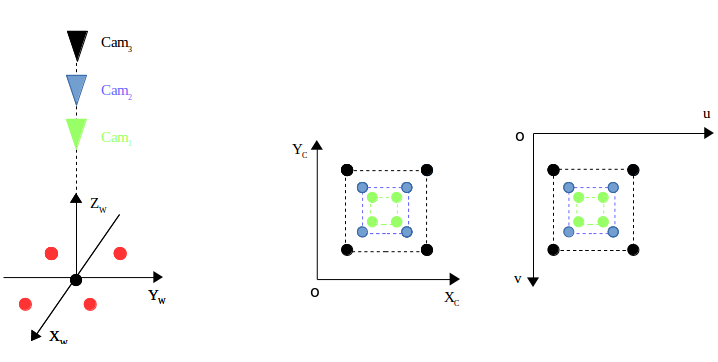
\includegraphics[scale=0.8]{./fig/cam123.png}
\caption{Test}  
\label{fig:cam123}
\end{figure}

\begin{figure}[H]
\centering
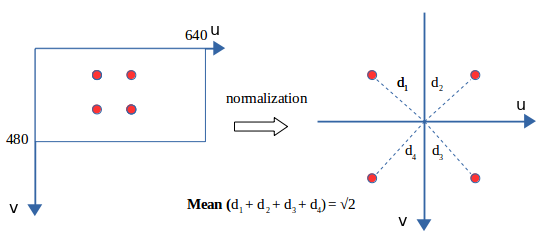
\includegraphics[scale=0.8]{./fig/normalization.png}
\caption{Normalization}  
\label{fig:normalization}
\end{figure}

\texttt{Condition number distribution with normalized homography(only translation but no scaling):}

We already know that we also need to consider the influence of the \texttt{height} on condition number. So we got one assumption: by normalization if we just implement the translation of the image points but not implement the scaling, maybe we we can get one ideal result. In order to verify this assumption we set the $scale = 1$ this times which means no scaling after translation of image points: 
\begin{python}\label{python:regular}
dist = []
pts = pts/pts[2, :]
for i in finiteind:
    c = np.mean(pts[0:2, i].T, axis=0).T
    newp1 = pts[0, i] - c[0]
    newp2 = pts[1, i] - c[1]
    dist.append(np.sqrt(newp1 ** 2 + newp2 ** 2))

dist = np.array(dist)
meandist = np.mean(dist)
scale = 1 # Only translation, no scaling
T = np.array([[scale, 0, -scale * c[0]], [0, scale, -scale * c[1]], [0, 0, 1]])
newpts = np.dot(T, pts)
return newpts,T
\end{python}

But obviously we got the result still with problem which is shown in figure \ref{fig:con_dis_Imag_OnlyTrans}. This figure shows that when the camera is closer to the marker, the condition number gets bigger. It is exactly the opposite of what we want.

The reason for this problem is that if the camera locates closer to the marker, the closer the four image points are to the origin of pixel coordinate. And according to the matrix \texttt{A} of condition number, if the image points locate closer to the origin of pixel coordinate, the smaller the condition number is. Therefore in this case we got a opposite conclusion.

\begin{figure}[H]
\hspace*{-4cm}
\centering
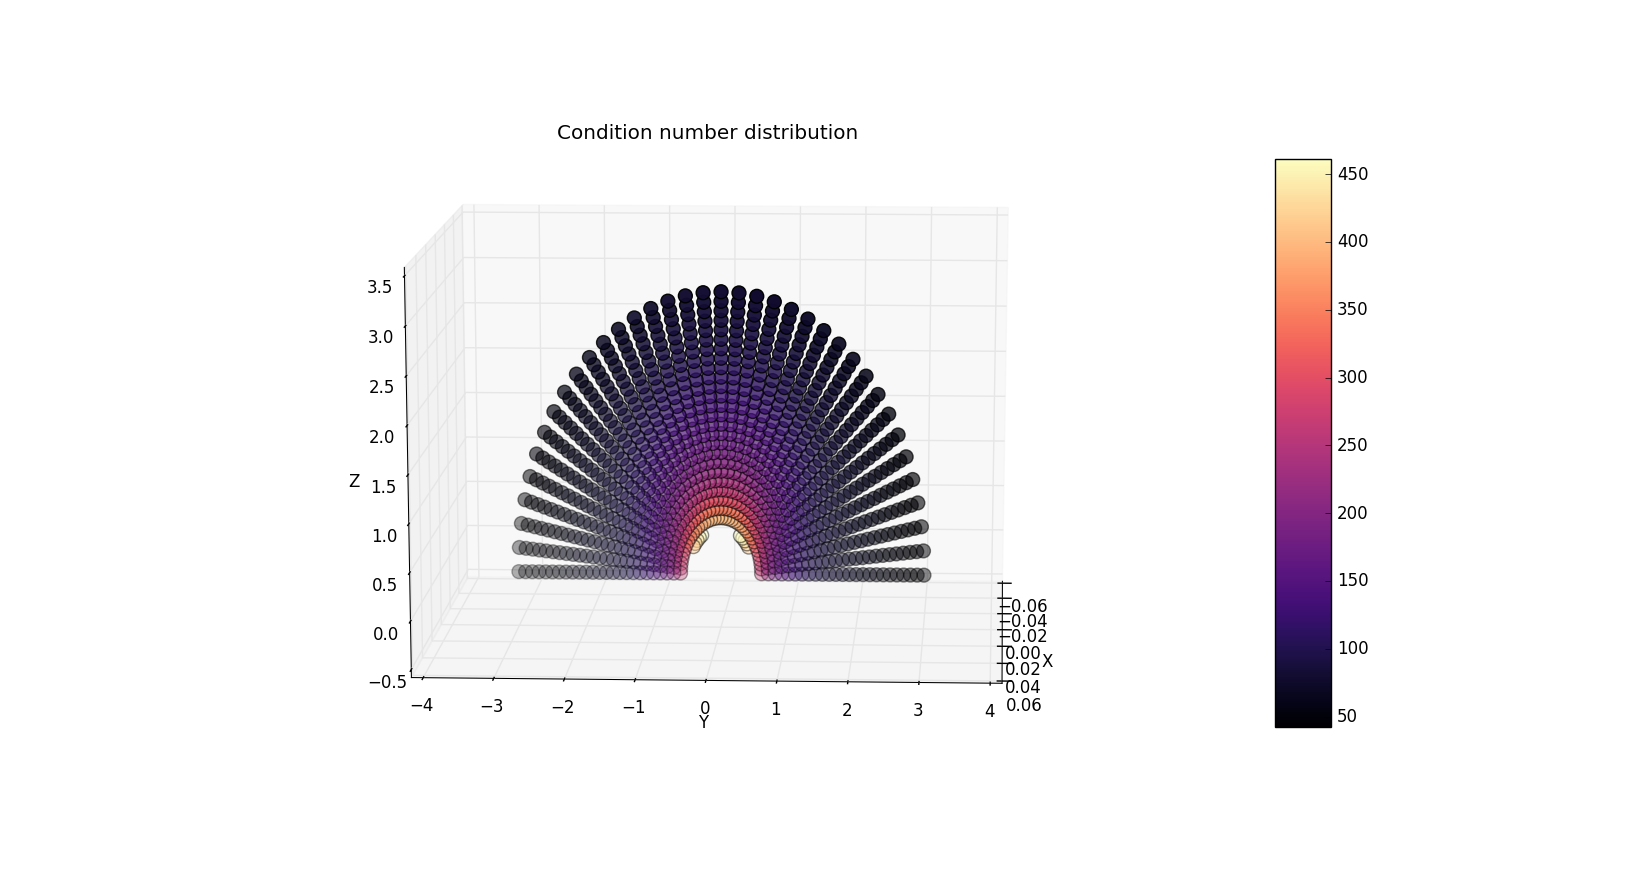
\includegraphics[scale=0.6]{./fig/con_dis_Imag_OnlyTrans.png}
\caption{Condition number distribution, object points are regular normalized and image points are normalized only with translation but no scaling(scale = 1)}  
\label{fig:con_dis_Imag_OnlyTrans}
\end{figure}

If in this case we got a opposite conclusion, can we just make a little trick that we set condition number as it's reciprocal?
\begin{python}\label{python:regular}
mat_cond = gd.matrix_condition_number_autograd(*input_list, normalize = normalized)
# TODO normalized with no scaling (scale = 1) , invert the condtion number
mat_cond = 1 / mat_cond
\end{python}

After performing this little trick, we found that the trend of condition number in terms of the change of \texttt{angle} is still not right, which is shown in figure \ref{fig:angleHeight_invert_condNum}(b). The reason is that before we applied the reciprocal of condition number, when the height is fixed, it has a lower condition number if the angle is smaller. Therefore when we applied the reciprocal of condition number, the lower angle has a bigger condition number.

\begin{figure}[H]
  \centering
  \begin{subfigure}[b]{1.0\textwidth}
    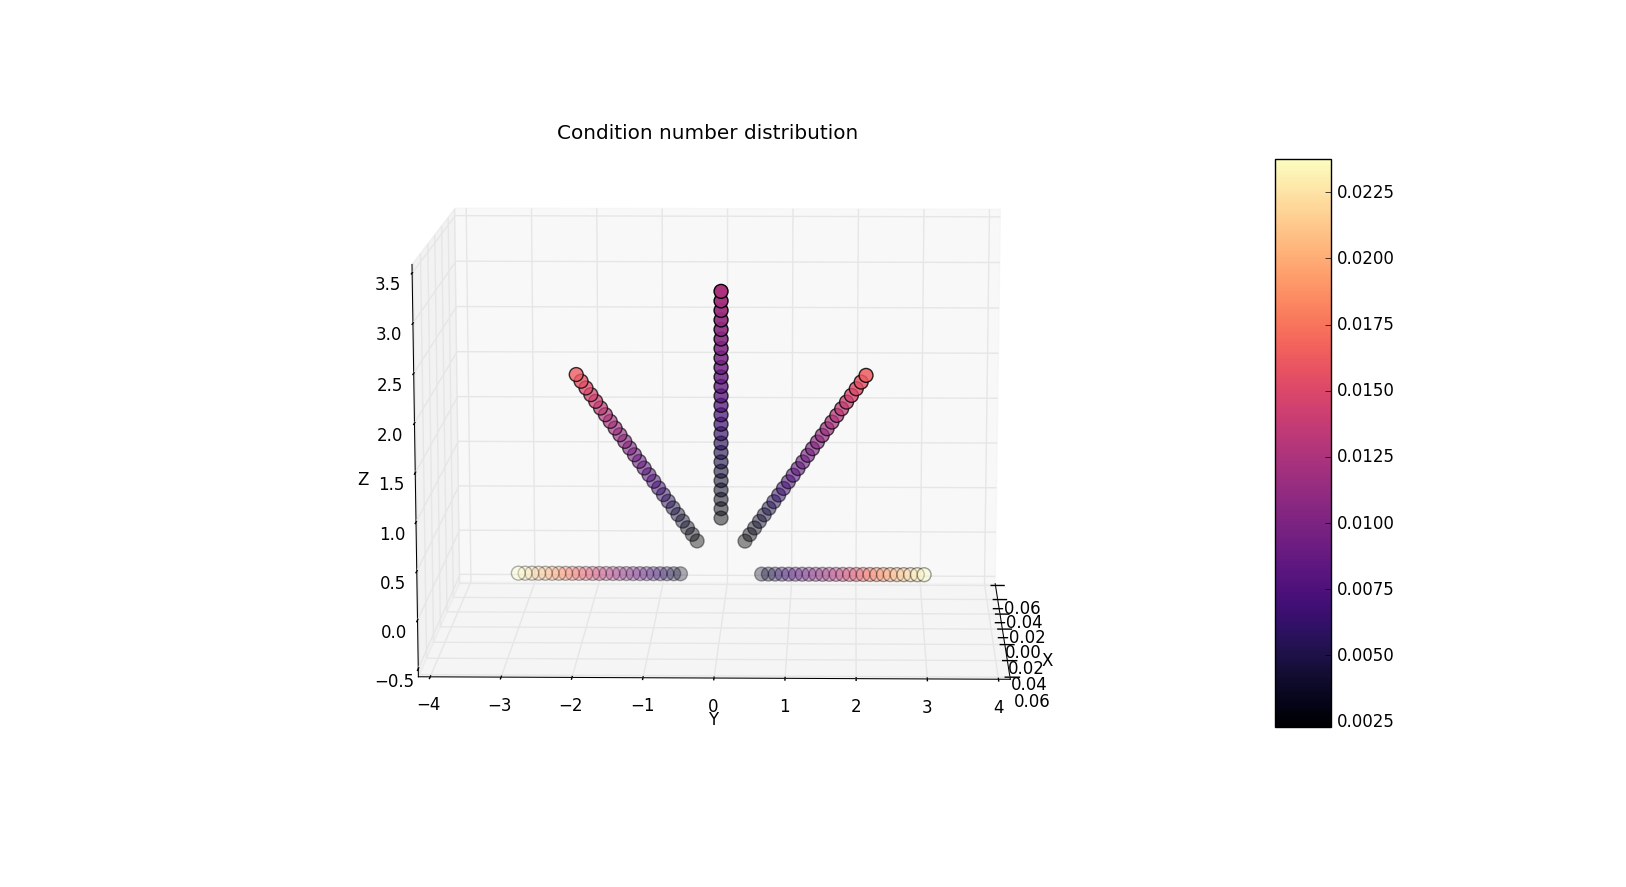
\includegraphics[width=\textwidth]{./fig/cond_num_dis_height.png}
    \caption{Condition number distribution when the angle is fixed as \SI{0}{\degree},\SI{45}{\degree},\SI{90}{\degree},\SI{135}{\degree} and \SI{180}{\degree}($condition number = 1/condition number $ }
  \end{subfigure}
  \begin{subfigure}[b]{1.0\textwidth}
    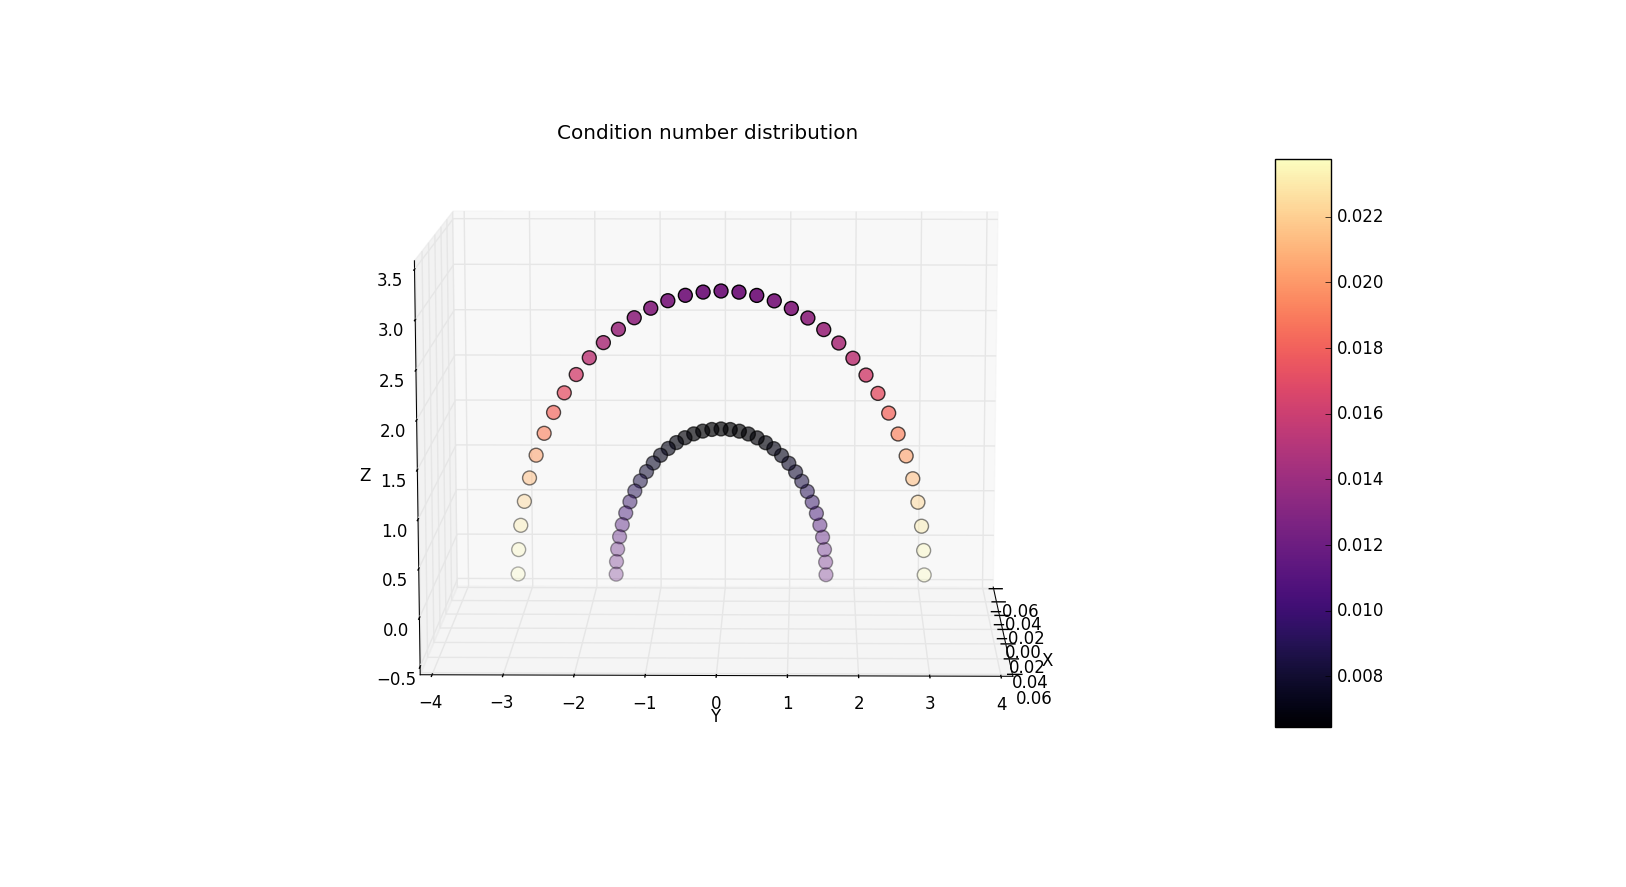
\includegraphics[width=\textwidth]{./fig/angle_invert_condNum.png}
    \caption{Condition number distribution when the height fixed at 1.55m and 3m($condition number = 1/condition number $}
  \end{subfigure}
  \caption{Condition number distribution of different camera positions, each circle represents each camera position, different colors represent different values(figure \ref{fig:magma})}
  \label{fig:angleHeight_invert_condNum}
\end{figure}  
  
\begin{figure}[H]
\hspace*{-4cm}
\centering
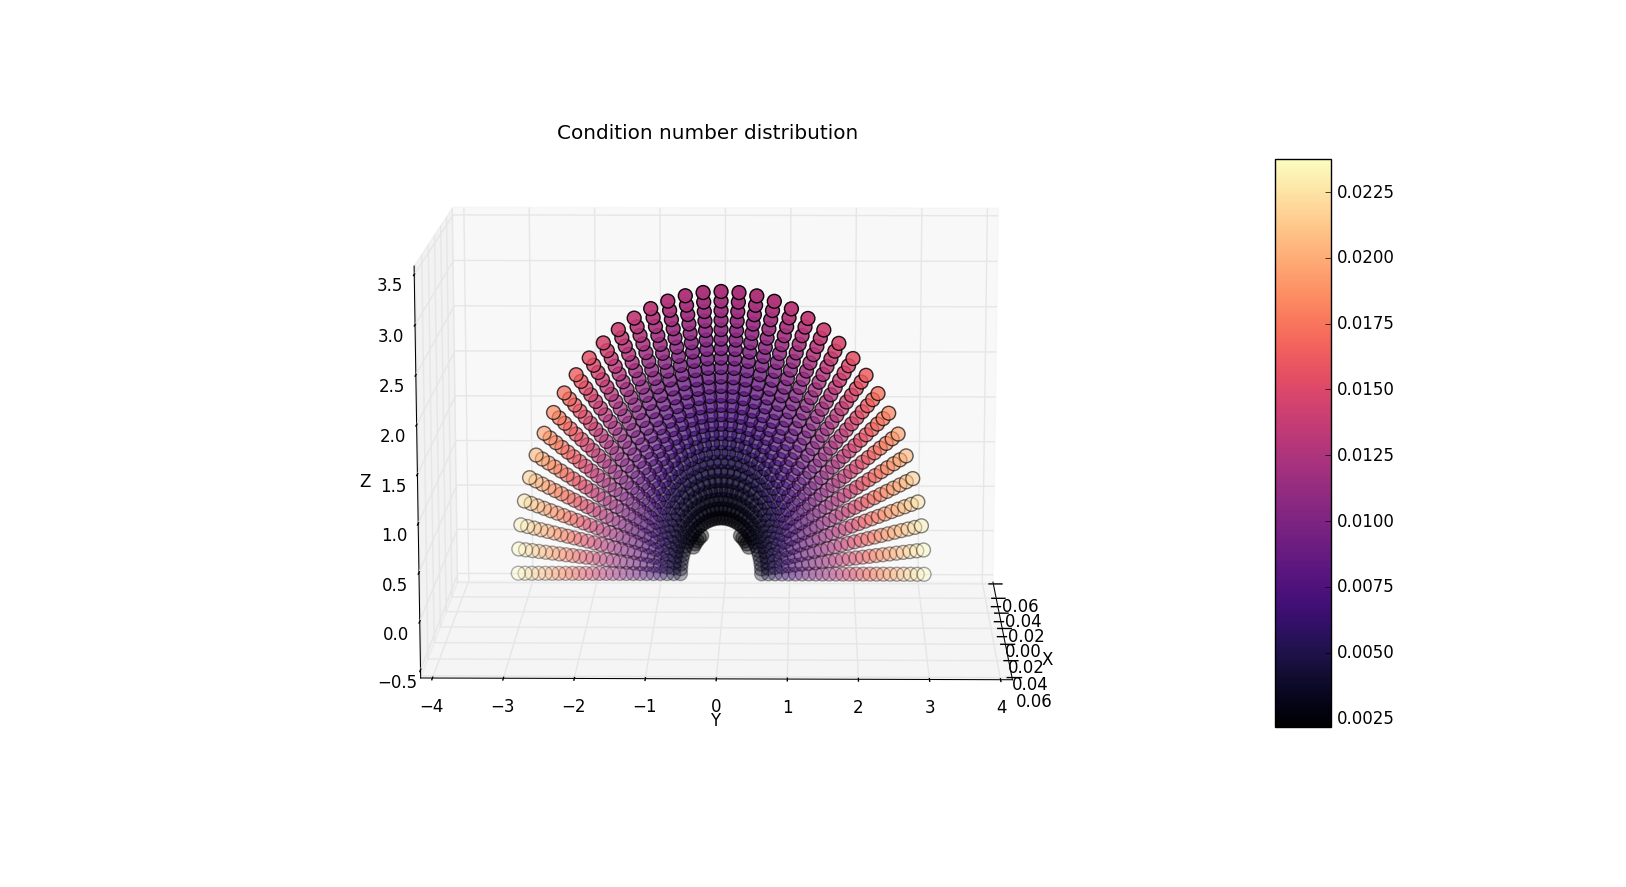
\includegraphics[scale=0.6]{./fig/invert_condNum.png}
\caption{Condition number distribution, object points are regular normalized and image points are normalized only with translation but no scaling(scale = 1), but $condition number = 1/condition number $}  
\label{fig:invert_condNum}
\end{figure}

\texttt{Condition number distribution with normalized homography(scale based on height):}

After all of these simulations, we used another trick: we set the product of height and regular normalized scale as the new scale of normalization:

\begin{python}\label{python:regular}
dist = []
pts = pts/pts[2, :]
for i in finiteind:
    c = np.mean(pts[0:2, i].T, axis=0).T
    newp1 = pts[0, i] - c[0]
    newp2 = pts[1, i] - c[1]
    dist.append(np.sqrt(newp1 ** 2 + newp2 ** 2))

dist = np.array(dist)
meandist = np.mean(dist)
scale = radius*np.sqrt(2)/meandist # Set the scale increasing with distance from camera to marker
T = np.array([[scale, 0, -scale * c[0]], [0, scale, -scale * c[1]], [0, 0, 1]])
newpts = np.dot(T, pts)
return newpts,T
\end{python}

And we got following desired results which are shown in figure \ref{fig:cond_num_Imag_Rnor_angleHeight}, this condition number distribution computed with this approach can be interpreted as the accuracy function.

\begin{figure}[H]
  \centering
  \begin{subfigure}[b]{1.0\textwidth}
    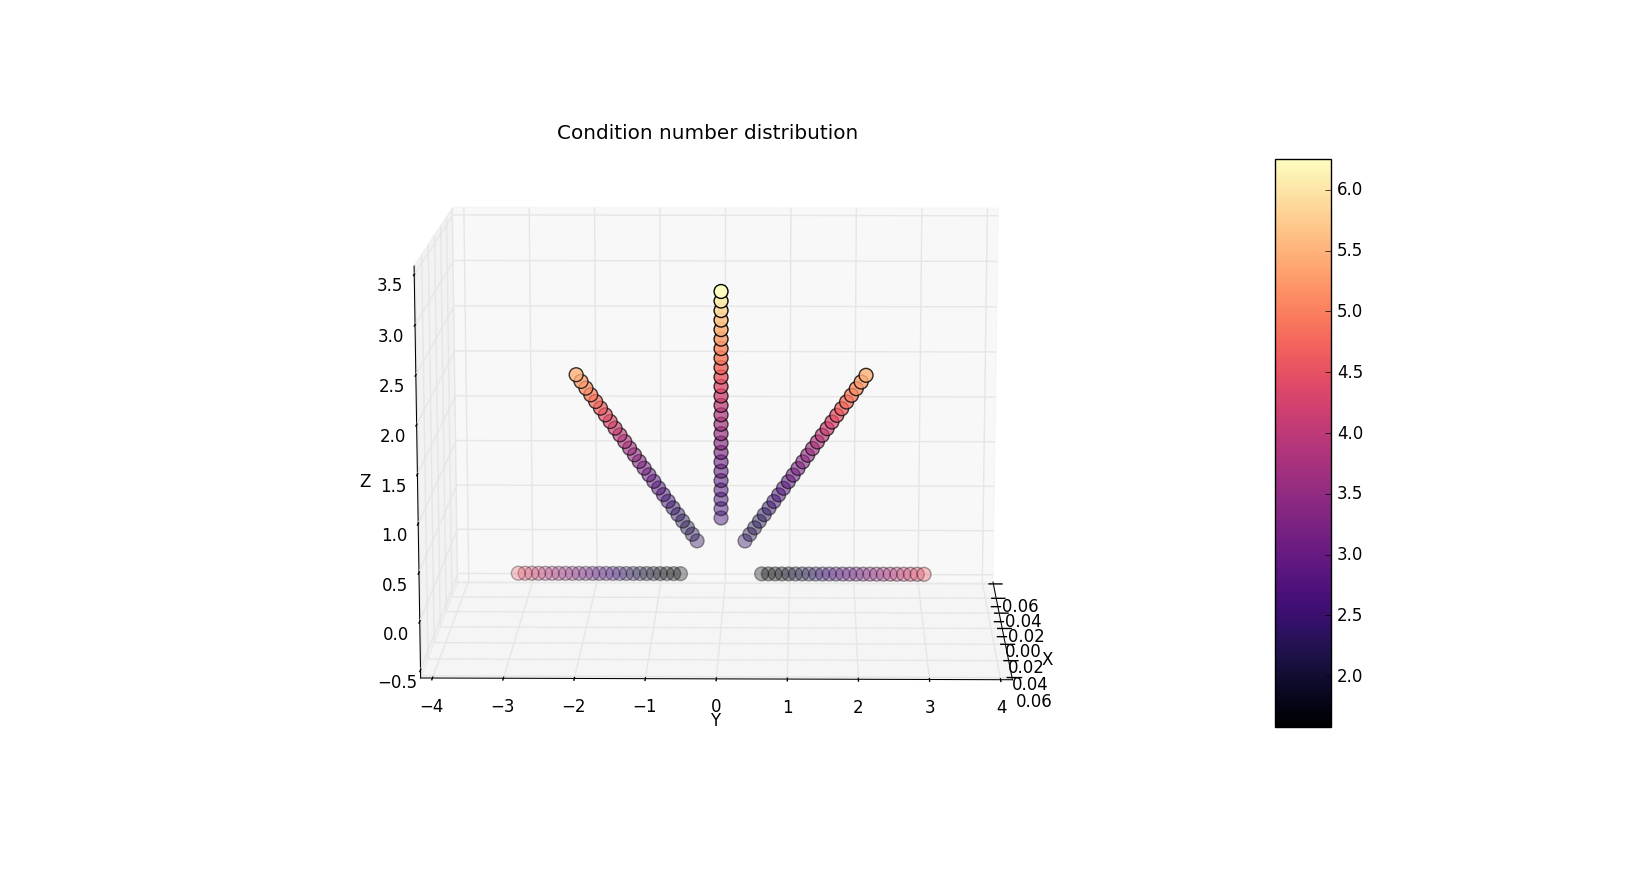
\includegraphics[width=\textwidth]{./fig/cond_num_Imag_Rnor_height.png}
    \caption{Condition number distribution, object points are regular normalized and image points are normalized with $scale = radius*np.sqrt(2) / meandist$. The angle is fixed as \SI{0}{\degree},\SI{45}{\degree},\SI{90}{\degree},\SI{135}{\degree} and \SI{180}{\degree}}
  \end{subfigure}
  \begin{subfigure}[b]{1.0\textwidth}
    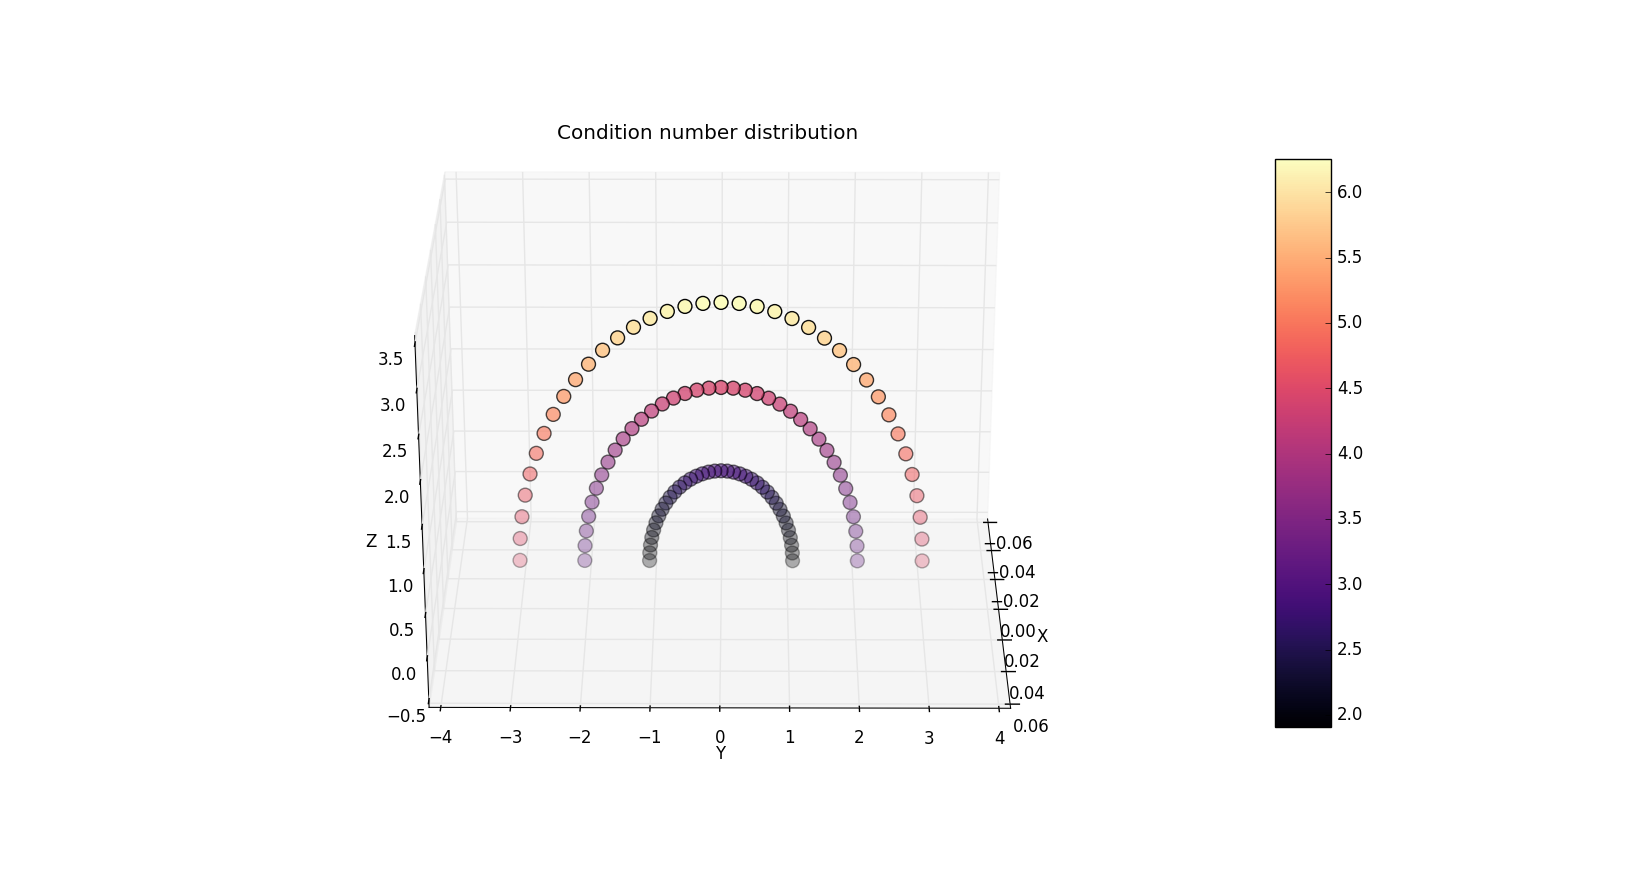
\includegraphics[width=\textwidth]{./fig/cond_num_Imag_Rnor_angle.png}
    \caption{Condition number distribution, object points are regular normalized and image points are normalized with $scale = radius*np.sqrt(2) / meandist$. The height is fixed as 1.06666667m, 2.0333333 and 3m}
  \end{subfigure}
  \caption{Condition number distribution of different camera positions, each circle represents each camera position, different colors represent different values(figure \ref{fig:magma})}
  \label{fig:cond_num_Imag_Rnor_angleHeight}
\end{figure}  

\begin{figure}[H]
\hspace*{-4cm}
\centering
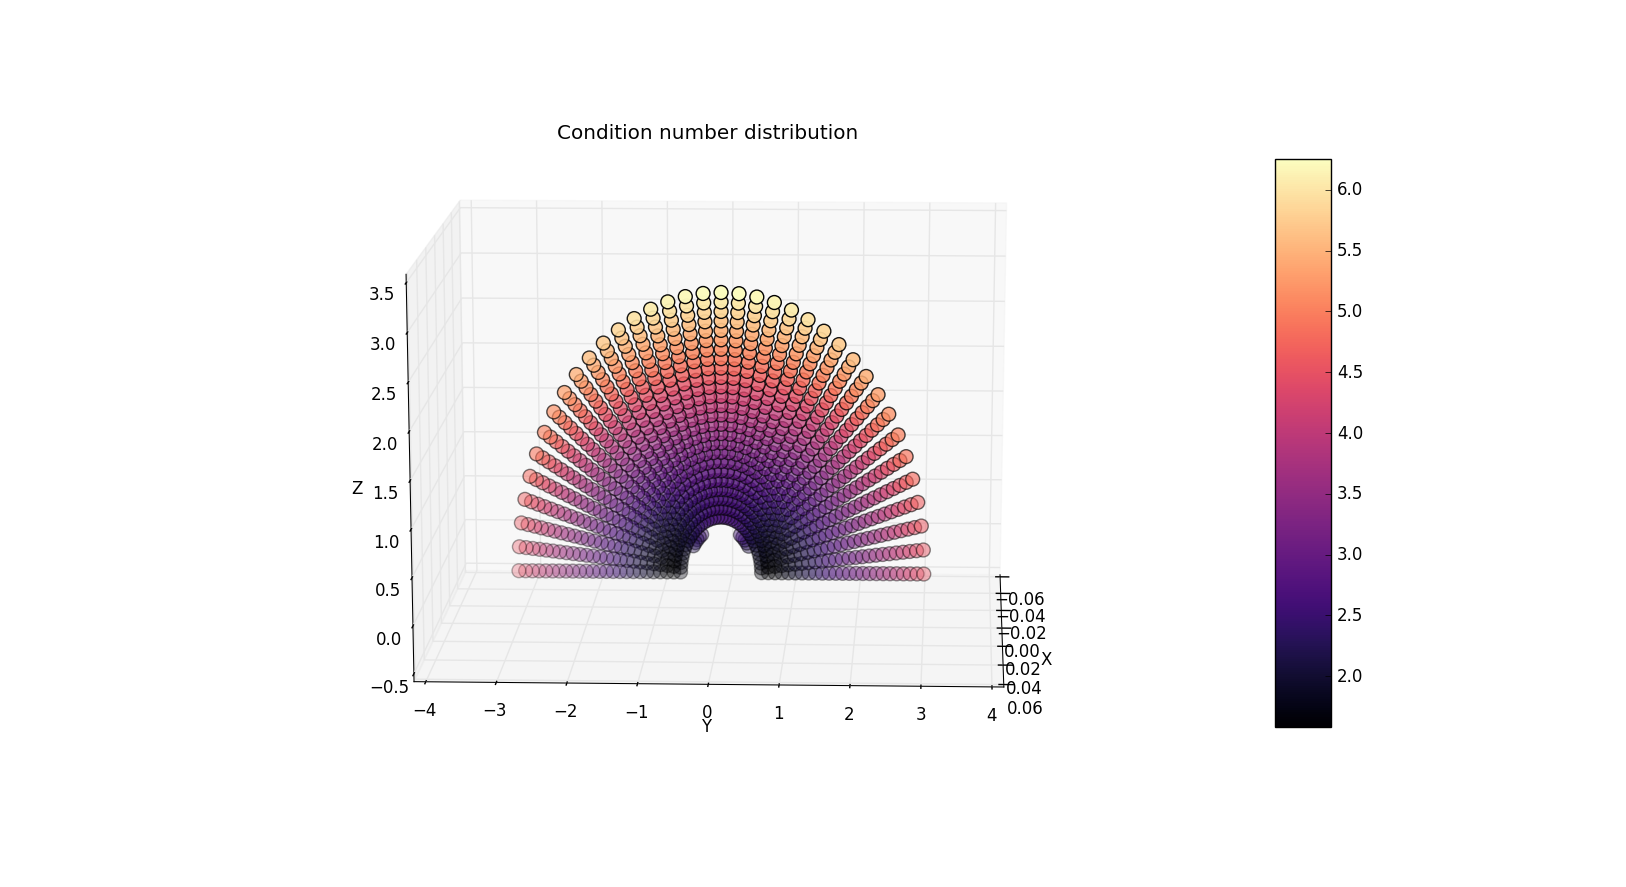
\includegraphics[scale=0.6]{./fig/cond_num_Imag_Rnor.png}
\caption{Condition number distribution, object points are regular normalized and image points are normalized with $scale = radius*np.sqrt(2) / meandist$}  
\label{fig:cond_num_Imag_Rnor}
\end{figure}

The figure \ref{fig:cond_num_Imag_Rnor_angleHeight}(a) shows the trend of condition number based on the change of \texttt{h}. We can find that when the camera is close to the origin of marker, it has a relative small condition number at this corresponding position. This is consistent with one of our desired results.

The figure \ref{fig:cond_num_Imag_Rnor_angleHeight}(b) shows the trend of condition number based on the change of \texttt{angle}. We can find that when the camera is close to the x-axis, it has a relative small condition number at this corresponding position. And the condition number distribution is exactly symmetrical. This is also consistent with another one of our desired results.\\

\texttt{Results summary:}

There is no doubt that normalization of homopraphy is an essential step to compute condition number of different camera positions for the accuracy function. However how to implement the meaningful normalization(e.g. how should the coordinates should be scaled?) is one step worth to think about.
 
After many simulations and considering different cases, we used one little trick to compute our desired condition number: we chose to scale the coordinates: the average distance of
a point x from the origin is equal to $radius \times \sqrt{2}$.

Using this little trick we got our desired results mentioned at the beginning of this section: 
The closer the camera is to the marker, the smaller the condition number is which means the more accurate the camera pose. However in the real case in view of the camera's detection range the camera can not be placed too close to the marker and the angle between the camera and the marker plane can not be too small. We can treat the condition number distribution as our accuracy function. Our results about condition number distribution were similar to the accuracy as a function of camera distance and relative camera angle in \cite{abawi2004accuracy} and \cite{pentenrieder2006analysis}.